% ------% % Uncomment and use as if needed
% \newtheorem{theorem}{Theorem}
% \newtheorem{lemma}[theorem]{Lemma}
% \newtheorem{proposition}[theorem]{Proposition}
% \newtheorem{definition}[theorem]{Definition}
% \newdefinition{remark}{Remark}
% \newtheorem{corollary}[theorem]{Corollary}

% %----------------New Commands---------------%
% \newcommand{\innerprod}[1]{\left\langle #1 \right\rangle}
% \newcommand{\abs}[1]{\lvert #1 \rvert}
% \newcommand{\bigabs}[1]{\left \lvert #1 \right \rvert}

% \newcommand{\sobkp}[1]{W^{k,p}(#1)}
% \newcommand{\sob}{W^{k,p}}
% \newcommand{\Lloc}[1]{L_1^{loc}(#1)}
% \newcommand{\totalV}[1]{D_t^{\abs{#1}}V(t)}
% \newcommand{\totalJ}[1]{D_t^{\abs{#1}}J(t)}
% \newcommand{\D}{\textbf{D}}
% \newcommand{\fhat}{\hat{f}}

% %minGW
% \newcommand{\argminpsi}{\min\limits_{g(\textbf{w}(t),\psi(t))\in \sob}}

% %minSmoothGW
% \newcommand{\minSmoothGW}{\min\limits_{g(\textbf{w}(t),\delta(\psi(t)))\in \sob}}


% \let\WriteBookmarks\relax
% \def\floatpagepagefraction{1}
% \def\textpagefraction{.001}

% % Short title
% \shorttitle{}    

% % Short author
% \shortauthors{}  

% % Main title of the paper
% \title [mode = title]{The Effect of Architechture on Learning Behavior of Deep Neural Networks}  

% % Title footnote mark
% % eg: \tnotemark[1]
% %\tnotemark[1] 

% % Title footnote 1.
% % eg: \tnotetext[1]{Title footnote text}
% \tnotetext[1]{} 

% % First author
% %
% % Options: Use if required
% % eg: \author[1,3]{Author Name}[type=editor,
% %       style=chinese,
% %       auid=000,
% %       bioid=1,
% %       prefix=Sir,
% %       orcid=0000-0000-0000-0000,
% %       facebook=<facebook id>,
% %       twitter=<twitter id>,
% %       linkedin=<linkedin id>,
% %       gplus=<gplus id>]

% \author[1]{Allyson Hahn}%[<options>]]

% % Corresponding author indication
% \cormark[1]

% % Footnote of the first author
% \fnmark[1]

% % Email id of the first author
% \ead{}

% % URL of the first author
% \ead[url]{}

% % Credit authorship
% % eg: \credit{Conceptualization of this study, Methodology, Software}
% \credit{}

% % Address/affiliation
% \affiliation[1]{organization={Department of Mathematical Sciences, Northern Illinois University}}

% \author[2]{Krishnan Raghavan}%[]

% % Footnote of the second author
% \fnmark[2]

% % Email id of the second author
% \ead{}

% % URL of the second author
% \ead[url]{}

% % Credit authorship
% \credit{}

% % Address/affiliation
% \affiliation[2]{organization={Mathematics and Computer Science Division, Argonne National Laboratory}}

% % Footnote text
% \fntext[1]{}

% % For a title note without a number/mark
% %\nonumnote{}

% %-------------------Abstract-----------------------%
% \begin{abstract}
% We consider the effects of Neural Network architecture in the setting of continual learning. Using dynamic programming we complete a bilevel optimization to determine the optimal architecture for the current and previous task data followed by the optimal weights for the network. 
% \end{abstract}

% % Use if graphical abstract is present
% %\begin{graphicalabstract}
% %\includegraphics{}
% %\end{graphicalabstract}

% %-----------------Highlights------------------%
% \begin{highlights}
% \item The first quantification of NN architecture on the learning behavior
% \item Demonstrate the conditions to ensure stability of neural networks.
% \item A novel measure to efficiently perform neural architecture search and hyper-parameter search.
% \end{highlights}
% %-------------------Keywords-------------------%
% \begin{keywords}
%  Neural Network \sep Architecture Search\sep  \sep
% \end{keywords}
% \maketitle
\section{Introduction}
With the advent of large scale AI models, the computational expense of training such model has also increased drastically; training these models efficiently often requires large scale high performance computing infrastructure. Despite such drastic expenditure, these models quickly become stale. This is because the data-distribution shifts or new data that gets generated as these model often drift~(become stale) due to change in the data distribution which requires realignment. This necessity presents a quandary. Naive realignment leads to a phenomenon called catastrophic forgetting where the model overwrites prior information. On the other hand, a complete retraining of the model would require significant resource and this solution is extremely unattractive. 

The more viable option is that of continual learning, where approaches seek to constrain the parameters of the model to reduce the amount of catastrophic forgetting the model experiences. Several works in the literature have attempted this direction, starting from early work on small multilayer perceptron~\cite{mccloskey1989catastrophic} to recent works on large language models such as \cite{luo2025empirical, lai2025reinforcement, biderman2024lora} and \cite{lin2025continual}. One key commonality across all of these approaches is that, they look to constrain the weight/parameters of the AI model to induce minimal forgetting. On the other hand, in some cases and more appropriately, many approaches seek to balance between forgetting and the learning on new data~(generalization) as in~\cite{raghavan2021formalizing, lu2025rethinking} and others~\cite{lin2023theory}. Despite demonstrated success, this is not the full story. In fact,  under mild assumptions, it has been proven that simply changing the weight of the AI model is not sufficient to capture the drift in the data distribution and the capacity of the NN~(its ability to represent tasks) eventually diverges if the data distribution keeps changing ~\cite{chakraborty2025understanding}. These intractability results from \cite{chakraborty2025understanding} highlight a conundrum, that is, if the capacity of the network eventually diverges, then, should we still aim to continually learn AI models even though continually learning such models is invaluable? \textit{In this paper, we demonstrate that the answer to this question is indeed ``yes," and, in fact, the solution is to reliably change the architecture of the AI model on the fly according to the need of the data distribution.} 

However, there are three key bottlenecks before attaining this goal: (i) reliably changing the architecture requires a methodical understanding of ``how the weights and the architecture of the model interact with each other," that is, the coupling between the weights and the architecture; (ii) moreover, to decide when to change the architecture, one must understand, ``how the forgetting-generalization trade-off is affected by the aforementioned coupling'. Loosely speaking, the first two bottlenecks have been heuristically attempted in the literature. For example, some recent works such as  CLEAS (Continual Learning with Efficient Architecture Search)~\cite{CLEASgao2022CLEAS} and SEAL (Searching Expandable Architectures for Incremental Learning)~\cite{SEALgambella2025SEAL} involves dynamically expanding the capacity of the AI model by adding layers and defining metrics that govern the necessity for a change in capacity. However, none of these approaches involve or enable a generic ability to change different aspects of the architecture, number of parameters, activation functions, layers, etc. The key reason is that, if the architecture is generically changed, one must initialize the new network architecture at random. (iii) Then, the transfer of information about the weights from the previous architecture to the new architecture across parameter spaces of two different shapes is required. However, this is currently impossible. In the absence of such a transfer mechanism, current approaches such as CLEAS and SEAL can only modify those components that would not warrant information transfer between parameter space of two different sizes. To address these bottlenecks, we will present a comprehensive approach that includes a novel formulation to understand the coupling between the architecture and the weights of the model, a methodical way of searching for a generic new architecture, and a novel method to transfer information between the old architecture and the new architecture.


\subsection{Contribution}
The key reason why the coupling between the architecture and the weights is difficult to model is because, architecture dependencies are observed on a function space across tasks and the weight dependencies are visible across the Euclidean parameter space. Any modeling in the weight space such as \cite{chakraborty2025understanding, raghavan2021formalizing} or \cite{lu2025rethinking} cannot capture function space dependencies. To obviate this, we model the problem of continually learning the AI model over a sequence of tasks in a Sobolev space. Using this theoretical framework, we describe, how in the Sobolev space of AI models, parameterized by architecture choices and the weights, weights alone cannot capture the change in the distribution and the architecture must be changed. We then employ a derivative free architecture search approach to determine the new architecture by searching for an appropriate number of neurons.  While in this work, we focus on changing the number of parameters in the AI model, our work is general enough to extend to other architecture choices as well. Once the new architecture is chosen, we develop a new algorithm that can efficiently transfer information from the previous architecture to a new architecture across parameter spaces of different sizes with minimal loss of performance on the previous tasks.

We then empirically demonstrate that changing the architecture indeed results in better training loss~(at least $\%$ more improvement) over the case where the architecture is not changed. We also show that our algorithm achieves substantial improvements~(upto $\%$) in terms of training loss when training over large number of tasks; is robust to noise~(Gaussian noise up to variance $\sigma =$) and scales from feedforward neural networks to graph neural networks seamlessly across regression and classification problems. We envision that jointly training the architecture and the weights in the continual learning paradigm is the best path to go forward in the field of continual learning and develop the basic theoretical and empirical infrastructure to allow for such training. 


\subsection{Organization}
The paper is organized as follows, we begin by a description on continual learning and motivate the necessity for function space modeling, then, we describe a collection of neural networks as functions in a Sobolev space. We then describe the impact of familiar and unfamiliar tasks on continual learning and describe the necessity to change the architecture along with the weights of the AI model. Finally, we describe the algorithm to change the architecture on the fly and transfer information between the two architectures. We finally describe empirically the advantages of our approach. 


\subsection{Notations}
These notation are adapted from \cite{kolda2009tensor}, please refer to the original paper for additional details. We use $\mathbb{N}$ to denote the set of natural numbers with $\mathbb{R}$ denoting the set of real numbers.  An $m^{th}$ order tensor is viewed as a multi-dimensional array contained in $\mathbb{R}^{I_1 \times I_2 \times I_3 \times I_4 \times \cdots I_{m}}$,  where the order can be thought of as the number of dimensions in the tensor. In this paper we will mostly be concerned with tensors of order $0, 1,2$ and $3$ which correspond to scalars, vectors, matrices, and a list of matrices. Therefore, we will write a tensor of order $0$; a scalar, with lowercase letters, i.e., $\sx;$  a tensor of order one is denoted by lowercase bold alphabets such as $\vx.$ A tensor of order $2$ is a matrix denoted by uppercase bold alphabets $\mx$ and any tensor of order greater than $2$ are denoted by bolder Euler scripts letters such as $\tx.$  We also use $\|.\|$ to denote the Euclidean norm for vectors, Frobenius norm for matrices and an appropriate tensor norm for tensors. Further, we will let $\innerprod{\cdot,\cdot}$ denote the dot product for vectors, matrices, or tensors. We will make one exception in our notation regarding the tensors that represent learnable/user defined parameters~(architecture, step-size/learning rate, etc.), we will denote these with Greek letters. The $i^{th}$ element of a vector $\vx$ is denoted by $\sx_{[i]},$ while the $(i,j)^{th}$ element of a matrix $\mx$ is denoted by $\sx_{[ij]}.$ Moreover, we denote the $i^{th}$ matrix in a tensor of order $3$ by $\mx_i.$  We will make the indices run from 1 to their capital letters such that $i = 1, \ldots, I.$ 


\section{Continual Learning -- Motivation}~\label{sec:motivation}
The problem of continual learning is that of an AI model learning a sequence of tasks. Here, we define a task as a set of data available to learn from. Without going into the specifics of the underlying space of an AI model, we will denote the AI model as $\hat{f}(\weight, \psi)$ where  $f$ denotes the composition of the weights$-\weight$ and the architecture$-\psi.$ We will define the particulars of these quantities in the later section; however, the key objective of this model is to learn a series of tasks. In this context, each task is represented by a data set obtained at a task instance, i.e. $t \in \tT, \tT = \{0,1,\ldots, T\}.$ We will assume that the dataset~(a list of matrices/vectors/graphs) represented by $\tx(t)$ are provided at each task $t\in \tT,$ where $\tx(t)$ is sampled according to the distribution $\mathbb{P}$ and $\tx(t) \subset \domain \subset \mathbb{R}^n$ such that $\domain$ -- the domain, is a measurable set with a non-empty interior. Moreover, $(\domain, \mathcal{B}(\domain), \mathbb{P})$ forms the probability triplet with $\mathcal{B}(\domain)$ being the Borel sigma algebra over the domain $\domain$. 
\begin{figure}
    \centering
    \includegraphics[width=\linewidth]{paperFigures/CL1.png}
    \caption{The basic problem of Continual Learning}
    \label{fig:CL1}
\end{figure}
The problem of interest to us is to understand the behavior of the AI model when it is learning on tasks $\tx(t)$ for every task instance $t.$ Notably, tasks instances can belong to $\mathbb{N}$ and $\mathbb{R}$ depending on the application at hand, but the key goal is to understand how the tasks are assimilated by the AI model. The basic notion of continual learning is described in Fig.~\ref{fig:CL1}, where there are three tasks at $t=1, 2$ and $3$. For each of these three tasks, an architecture $\psi(1)$ is chosen and the three tasks are provided to the model in series. At $t=1$, the model $\hat{f}$ learns from the first task. In particular, we solve the optimization problem 
\begin{align}
min_{\weight(1)} \ell(\hat{f}(\weight(1), \psi(1)), \tx(1))
\end{align}
where $\ell$ is some loss function that summarizes the models performance on the task at $t=1.$ Then, at $t=2,$ the model transfers to learn information from the second task such that the first task is not forgotten. Implicitly, the optimization problem is rewritten as 
\begin{align}
    min_{\weight(2)} \left[ \ell(\hat{f}(\weight(2), \psi(1)), \tx(1)) + \ell(\hat{f}(\weight(2), \psi(1)), \tx(2)) \right] 
\end{align}
Similarly, at $t=3,$ the model transfers to learn information from the third task, but both tasks 1 and 2 must not be forgotten. This implies that 
\begin{align}
    min_{\weight(3)} \left[ \ell(\hat{f}(\weight(3), \psi(1)), \tx(1)) + \ell(\hat{f}(\weight(3), \psi(1)), \tx(2)) + \ell(\hat{f}(\weight(3), \psi(1)), \tx(3))\right] 
\end{align}
As evidenced the objective of the model is to remember all earlier tasks. Notably, this implies that the objective function of the continual learning problem is a sum that grows with every new task. Therefore, at any task $t,$ the objective of the CL problem is 
\begin{align}~\label{eq:CL_for}\tag{Forgetting Loss}
    min_{\weight(t)} \sum_{i=1}^t \left[\ell(\hat{f}(\weight(i), \psi), \tx(i)) \right] 
\end{align}
where we have removed the index from $\psi$ to indicate that the architecture is fixed. In the CL literature, \eqref{eq:CL_for} is typically optimized at the onset of every new task at $t.$ The most rudimentary approach for optimization of  \eqref{eq:CL_for} is conducted through an experience replay array that maintains a memory of all tasks in the past. To gain more insight into what happens at the onset of each new task, observe Figure \ref{fig:param}.

\begin{figure}[!htb]
    \centering
    \includegraphics[width=0.6\linewidth]{Figures/par_space.png}
    \caption{The basic problem of Continual Learning}
    \label{fig:param}
\end{figure}
For the sake of illustration, we assume that $\ell(\hat{f}(\weight(i), \psi, \tx(i))$ is a strongly convex function and describe in Figure ~\ref{fig:param}, the level set~(the balls) in the parameter space corresponding to $\ell(\hat{f}(\weight(i), \psi, \tx(i)) \leq \eta$  and the plus sign corresponds to the minima for $i=1$ and $i=2.$ Notably, $\eta$ is the threshold to identify acceptable loss values and defines the boundary of the level set and by extension, the radius of the ball in Figure~\ref{fig:param}.  For instance, in the case of MNIST dataset, the two balls may represent two tasks of representing digit 0 and digit 1. The boundary of the left ball represents all parameters that provide cross entropy loss less than $\eta=1$ for digit 0  with the plus sign representing zero cross-entropy loss. Similarly, the right ball represents all parameters that provide cross entropy loss less than $\eta=1$ for digit 1 and the plus sign corresponds to zero cross entropy loss on digit 1. Within this example, consider an AI model~(maybe a CNN)  that trains on digit zero and achieves zero loss on digit zero, that is, attain the plus sign in the parameter space. Then, the AI model starts training for the next task- digit 1. First it starts from the plus sign achieved for digit 0, this implies that, there is an inherent bias due to the local minima achieved for digit 0. Second, when the new task is observed the model must converge to a solution that is common to both digit 0 and digit 1. This solution is trivial if the digit 0 and 1 were identical or very close to each other. However, as this is not the case, the solution must lie in the intersection between the two balls, that is, the region of the smiley face. Since the size of the intersection space depends on how different tasks 0 and 1 are, the following informally stated theorem is observed.

\begin{theorem} 
\label{thm:task_nonstationary_weights}
 Fix the number of weight updates required to obtain the optimal value at each task. Assume that each subsequent task introduces a value of change into the model with the change described in some appropriate metric. Let $\ell$ be the Lipschitz continuous and choose a small learning rate. Then, capacity diverges as a function of number of tasks.
 \textbf{Please see \cite{chakraborty2025understanding} for a full statement and its proof}
\end{theorem}

The theorem implies that, the AI models' ability to successfully represent tasks will deteriorate as more tasks are introduced when the new tasks are different from the previous one. In such case, continually learning the AI model is bound to fail if we just update the weights of the network. In this paper, we hypothesize that size of the intersection space in Figure.~\ref{fig:param} can be increased by modifying the architecture of the AI model, that is, by increasing the number parameters in the model. However, increasing the number of parameters would require us to model the coupling between the weights, data, and the architecture, which is impossible to imagine with the intuition laid out until now as this \textcolor{red}{intuition corresponds to a Euclidean} \Ally{what do you mean by this? Is it "Euclidean space" or am I misunderstanding?} where the notion of architecture cannot be modeled. To this end, we will describe a neural network as a member of a class of functions in a function space which we choose to be a Sobolev space.


\section{Neural Networks belong to a class of Sobolev space functions}
The goal of this section is to formalize the mathematical modeling required to identify the dependency between the intersection space from Figure.~\ref{fig:param}, the architecture and the AI model. Towards this end, we first define the AI model $\hat{f}(\weight, \psi)$ to belong to a class of functions contained in a Sobolev space with $k$ bounded weak-derivatives. The notion of $k$ bounded weak derivative is the key reason why Sobolev space is an appropriate choice for this problem, which we will discuss once we outline the formal definitions of Sobolev space aligning with definitions provided in \cite{mahanNonclosednessSetsNeural2021a} Therefore,
\begin{definition}\label{defn:sobo}
    Let $k \in \mathbb{N},$ the domain-$\domain \subset \mathbb{R}^n$ a measurable set with non-empty interior, and $1< p < \infty.$ Then, the Sobolev space $\sobolev$ consists of all functions $f$ on $\domain$ such that for all multi-indices $\alpha$ with $|\alpha| \leq k,$ the mixed partial derivative $\partial^{(\alpha)} f$ exists in the weak sense and belongs to $L^p(\domain)$. That is, 
    \[ \sobolev  = \{ f \in L^p(\domain) : \partial^{|\alpha|} h \in L^{p}(\domain) \forall |\alpha| \leq k \}.\]
    The number $k$ is the order of the Sobolev space and the Sobolev space norm is defined as 
    \[ \|f\|_{\sobolev} := \sum_{ |\alpha| \leq k } \| \partial^{|\alpha|} f \|_{L^{p}(\domain)}.\]
\end{definition}
\Ally{Need to revisit first half of this paragraph. Heine-Borel gives compact if and only if closed and bounded. So, should we flip this part by saying it is only practical to assume we have a finite set which is automatically closed and bounded and hence compact? What is currently here, to me, sounds like "because it is a subset of $\rn$ we can assume it is compact and closed by H-B," which is not true. Additionally, a "domain" is an open and connected subset. In this context, do we mean "domain" in the sense of "points which can be inputs" rather than the topological definition? If so, is this something the audience knows?}
In definition \ref{defn:sobo}, two key notions must be highlighted. First, the $\domain$ is by definition a subset of $\rn,$ which by virtue of the Heine-Borel Theorem~\cite{rudin1976principles}, is compact and closed. The implications of this assumption are important to consider. $\domain$, in this context is the data sample space and therefore, the assumption of compact and closedness applies to the data space. For any standard AI applications, this assumption implies that the data space is finite and the numerical values are bounded. Both are notable practical considerations that must be followed in any AI model training as it is well known that the without normalization, the AI model training fails to converge~\cite{huang2023normalization}. Therefore, this assumption is not only practical but necessary. The next assumption is presence of weak derivatives, notably, in the case of standard neural network, derivatives are assumed to exist as twice differentiability is necessary for training and typical training involves gradient based methods~\cite{kingmaAdamMethodStochastic2017}. In fact, the existence of weak derivatives can be summarized for different activation functions as in Table~\ref{tab:Sobolev_acti}. As noted in the table, all standard activation functions can be recast in the purview of definition~\ref{defn:sobo} and a Sobolev space can be constructed, that represents the class of functions that can be approximated by neural networks. The appropriateness of approximation and the condition over which such approximations are possible is discussed in \cite{petersenTopologicalPropertiesSet2021a}  and \cite{adegokeHigherDerivativesInverse2016}.
\begin{table}[!tb]
\adjustbox{max width=\linewidth}{
\begin{tabular}{cccc}
\toprule
       Name  &  $\rho(\vx)$ &  Smoothness & Corresponsding $W^{k,p}$\\
        &   & /Boundedness & \\
       \hline  \hline
Rectified Linear  & $max\{0,\vx\}$ & absolutely  & $W^{0,p}(\domain)$ \\
 Unit (ReLU) &  &  continuous, $\rho' \in L^{p}(\domain)$ & 
\\ & &  &\\ 
 Exponential Linear  & $ \vx. \chi_{\vx\geq 0}$ & $C^1(\mathbb{R})$, absolutely  & $W^{1,p}(\domain)$ \\
 Unit (eLU) & $+ (e^{\vx}-1) \chi_{\vx<0} $  & continuous $\rho'' \in L^{p}(\domain)$ & 
\\ & & &  \\ 
Softsign & $\frac{\vx}{1+ |\vx|}$ & $C^1(\mathbb{R})$, $\rho'$ absolutely  & $W^{2,p}$  \\
& &  continuous, $\rho'' \in L^{p}(\domain)$ &  
\\ & & &  \\ 
Inverse Square  & $ \vx \chi_{\vx \geq 0}  $ & $C^2(\mathbb{R})$, $\rho''$ absolutely  & $W^{3,p}$  \\ 
Root Linear Unit & $ + \frac{\vx}{\sqrt{1+a\vx^2}} \chi_{\vx<0} $ & continuous, $\rho''' \in L^{p}(\domain)$ & 
\\ & & &  \\ 
Inverse Square Root Unit & $ \frac{\vx}{\sqrt{1+a\vx^2}} $ & real analytic,  & $W^{k,p} \forall k $ \\
&  & real all derivatives bounded &  
\\ & & &  \\ 
Sigmoid & $ \frac{1}{1+ e^{\vx} } $ & real analytic,  & $W^{k,p} \forall k $ \\
&  & real all derivatives bounded &  
\\ & & &  \\ 
tanh & $ \frac{e^{\vx} - e^{-\vx}}{e^{\vx} + e^{-\vx}} $ & real analytic,  & $W^{k,p} \forall k $ \\
&  & real all derivatives bounded &  \\
\bottomrule
\end{tabular}
}
\caption{Different activation functions and the corresponding Sobolev spaces. Many of these results are described in the following references, 
\cite{petersenTopologicalPropertiesSet2021a}  and \cite{adegokeHigherDerivativesInverse2016} for details. $\chi$ is an indicator function.}
\label{tab:Sobolev_acti}
\end{table}

To represent the class of functions described in Definition \ref{defn:sobo}, we will define a neural network as a function  $\fhat(\weight(t),  \psi(t) )$ with $d \in \mathbb{N}$ layers. In this notation of a neural network, $\weight(t)$ is a long $\mathbb{R}^{m}$ vector that concatenates the weight parameters from the $d$ layers, and $\psi(t)$ is comprised of the architecture and other user-defined parameters that are present in the neural network.
\begin{definition} \label{defn:NN}
A $d$  layered neural network is given by an operator~(essentially a function) 
$\fhat(\weight(t), \psi(t) )\in \sobolev$ with $\sobolev$ being a Sobolev space. Furthermore, 
\begin{align}
  \fhat(\weight(t), \psi(t)) \big( . \big) & = \fhat_{d}(\mathrm{w}_{d}(t), \psi_{d}(t))\circ \fhat_{d-1}(\mathrm{w}_{d-1}(t), \psi_{d-1}(t))\circ \cdots \circ \fhat_{2}(\mathrm{w}_{2}(t), \psi_{2}(t))\circ \fhat_{1}(\mathrm{w}_{1}(t), \psi_{1}(t)) \big( . \big)
\end{align}
describes the layer-wise compositions and $\big( . \big)$ represents the input tensor to which the operator is applied.
\end{definition}
\begin{remark}
    Notation wise, we indicate approximate quantities with $\hat{.}$ and true~(target) quantities without the hat. For instance, the target function $f$ in definition~\ref{defn:sobo} is indicated without the hat and the approximate function $\fhat$ in definition~\ref{defn:NN} is indicated with a hat.
\end{remark}
\begin{remark}
    In definition~\ref{defn:NN}, we describe the operation across different layers using the composition, notation wise, we hide this complexity through the definition of the operator. Due to this, definition~\ref{defn:NN} is generic and  can be used to define feedforward neural networks, recurrent, convolutional, graph neural networks and even a large language model. Therefore, any analysis from this point is applicable to all types of neural networks. 
\end{remark}
Typically, the user-defined parameters are a combination of integer, categorical, and floating point values and we assume that the architecture can be varied with task instances. Therefore, the parameters corresponding to the architecture $\psi$ are assumed to be a function of the task instance $t.$
As we cannot determine derivatives with respect to discrete parameters in the classical sense (i.e., derivative of $\psi(t)$), we will need to define weak derivative with respect to these quantities such that the derivatives~(with respect to or of $\psi$) can be approximated. To describe the learning problem, we define a notion of loss function on the space of functions defined in definition~\ref{defn:NN} and \ref{defn:sobo}. 
 \begin{definition}\label{defn:NN_learning}
        Let $f(t)\in \sobolev$ for all $t\in \{0,\ldots, T\}$ denote the \textit{target function} which is to be approximated and let $\hat{f}(\weight(t),\psi(t))$ denotes a neural network determined to approximate $f(t)$ at task $t,$ then the \textit{loss function} (or error of approximation) for $\vx \in \tx(t) \subseteq \domain$ is given by 
        \begin{align*}
            \ell(\fhat(\weight(t),\psi(t)), \vx) & = \| \fhat(\weight(t),\psi(t))(\vx)-f(t)(\vx)\|_{\sobolev}.
        \end{align*} 
    \end{definition}
The function $f$ in the context of ML is an ideal forecasting model that can forecast temperature perfectly or an ideal classification model that performs some classification problem.
\begin{remark}
    In applications, we will assume $\domain$ is compact to guarantee the target function $f(t)$ exists in a Sobolev space $\sobolev,$ by Corollary 3.5. in \cite{mahanNonclosednessSetsNeural2021a}. However, in the event compactness cannot be assumed, we find the minimum norm solution to the problem in the Sobolev space.
\end{remark}
The loss function in definition~\ref{defn:NN_learning} is defined over $\sobolev$ using the Sobolev space norm. However, in practice, we can directly utilize samples corresponding to $f$ or $\hat{f}$ to construct the loss function from samples. For instance, this has been done in \cite{son2021sobolev} in the context of physics informed neural network - a class of neural networks that are modeled by definition~\ref{defn:NN}. In particular, the sobolev space norm is defined as in definition~\ref{defn:sobo}, where the loss function is a sum over $L^p$ norm over all $k$ weak derivative. As a trivial case, choosing $k=0$ and $p=2$ gives the standard mean squared error loss function which according to  Table~\ref{tab:Sobolev_acti} and practical consideration is applicable to variety of activation functions used in practical AI.

\subsection{Continual Learning in $\sobolev$}
Extending definition~\ref{defn:NN_learning} to the case of continual learning will provide us with the objective to optimize. As described in \ref{sec:motivation}, the goal of CL is to learn over a series of tasks such that the prior tasks are not forgotten. In particular, for each task instance $t,$ we must find $\weight$ that is optimal with respect to an objective function $J$ defined over the interval $[0,t].$ This objective function is known as the forgetting loss and was informally defined in \eqref{eq:CL_for}. Specifically, we rewrite \eqref{eq:CL_for} in terms of data, weights, and architecture, as below
\begin{align*}
    J(\weight(t),\psi(t),\tx(t)) & = \int_0^t \left( \int_{\vx \in \tx(\tau)} \ell(\fhat(\weight(t),\psi(t))( \vx ) ) \right) \;  d~\tau
\end{align*}
A traditional learning structure seeks to minimize the cost $J(t)$ through an iterative 
procedure that drives $J(t) \rightarrow 0$ as $t \rightarrow \infty$ iff $\tx(t_1) = \tx(t_2), \forall \; t_1, t_2 \in [0,T].$  This learning  structure is also mathematically guaranteed to converge with standard optimizers such as 
Adam~\cite{kingmaAdamMethodStochastic2017}. However, since $\tx(t_1) \ne \tx(t_2), \forall \; t_1, t_2 \in [0,T],$ we encounter the issue described in Figure~\ref{fig:param}. As described in section~\ref{sec:motivation}, there exists an inherent bias due to the order in which the tasks are observed and every time a new task is obtained, the underlying optimization problem needs to be resolved. In particular, we obtain a series of optimization problems corresponding to a series of tasks which leads to a dynamic program~\cite{bertsekas2012dynamic} over the target functions for each task. Typically, such dynamic programs~\cite{bertsekas2012dynamic} are solved by writing a cumulative optimization problem over the interval $[0,T]$ as in 
\begin{align*}
    V^*(t,\weight(t)) & = \min_{\weight \in \mathcal{W}(\psi^*(t))} V(t,\weight(t)),
\end{align*}
where $\mathcal{W}(\psi^*(t))$ is the weights search space, and $V(t,\weight(t))$ is given below
\begin{align*}
    V(t,\weight(t)) & = \int_t^T J(\weight(\tau),\psi^*(t), \tx(\tau)).
\end{align*}
A typical learning process is provided in  \cite{raghavan2021formalizing, chakraborty2025understanding} for these approaches 
involve extracting batches of data from $\tx(t)$ and then updating the network 
based on these batches of data. All of these updates are performed with a fixed architecture~$\psi^*(t)$. 
However, we are instead interested in the scenario where  the architecture and the model parameters are both learned. 
In order to learn the optimal weights and architecture for our network for all tasks, we must complete a bilevel optimization. First, we determine the optimal architecture, denoted $\psi^*(t)$ for the $t$th task. This optimization is completed below
\begin{align}\label{eq:arch} \tag{Architecture search}
    \psi^*(t) & = \mathrm{arg }\min_{\psi\in \Psi} J(\weight(t),\psi,\tx(t)),
\end{align}
where $\Psi$ is our architecture search space. Once completed, we move to the lower level optimization of the weights by utilizing dynamic programming. We determine  
\begin{align}\label{eq:clcum} \tag{Cumulative CL}
     V^*(t,\weight(t)) & = \min_{\weight \in \mathcal{W}(\psi^*(t))} V(t,\weight(t)),
\end{align}
This provides a holistic view of a learning problem for all tasks which incorporates the impact of architecture and weights.
As discussed in the introduction, naively solving this problem will involve repeatedly retraining the model from scratch for each new task. This is both computationally and mathematically unattractive. Therefore, we seek to find an elegant solution to this problem and to do this, we must understand the effect of subsequent tasks on the CL learning problem and by extension the effect of architecture on the CL problem.


\section{Understanding the existence of the CL solution}
For illustration, let us reconsider the example from 
section~\ref{sec:motivation}. In this regard,
we draw Figure ~\ref{fig:challenge}
where three tasks are shown to the model in order and the 
architecture of the network is fixed as $\psi(1).$ The goal of the 
CL is to solve the problem in 
\eqref{eq:clcum} at each task $t$ such that optimal weights 
can be determined. However, determining the optimal weights 
is highly dependent on each task's data. Intuitively, 
if the data in task $\tx(t) = \tx(t+1), \forall \; t \in [0,T],$ 
we can find a NN $\hat{f}$ which learns the new task $\tx(t+1)$
and transfers learning 
from $\tx(t)$ perfectly. But, if  
$\tx(t) \ne \tx(t+1), \forall \; t \in [0,T],$ 
we may or may not be able to find a common solution.

\begin{figure}[!thb]
    \centering
    \includegraphics[width=0.8\linewidth]{paperFigures/problem1.png}
    \caption{The actual problem}
    \label{fig:challenge}
\end{figure}
To illustrate this further, consider 
Figure  \ref{fig:challenge} and 
let $\mathcal{F}_t = \{\fhat(\weight,\psi)\in \sobolev\}$ 
to represent the search space for the set of 
all possible NN solutions for learning task 
$t$~(refer to  \ref{sec:motivation} for a similar construction). 
As $\mathcal{F}_t$ is a subset of $\sobolev,$ the balls in Figure  \ref{fig:challenge} 
can be thought  of as a representative of a level set such that the boundary of the size
of the ball represents the set of all solutions that provide the 
loss value less than a threshold. 
At $t=1$, there is one ball, at task $t=2$ there are two balls, 
and at task $t=3$ there are three balls. 
The number of balls here correspond to the number of tasks being 
involved in the learning process at each step of learning. 
 
In each of the balls, \ding{58} represents the NN solution for 
only that particular task $t$ and the smileys face 
represents the solution that transfers learning amongst tasks 
between $0$ to $t.$  Notably,  $\smiley{}$ must lie in 
the intersection of all the balls, as 
solution common to tasks $0$ to $t$ are only available in this 
intersection. Curiously, unless the tasks as equivalent, the $\smiley{}$ 
and the \ding{58} will not coincide because no solution 
that is perfect for one task ends up being perfect for another. 
Furthermore, the more different the subsequent tasks are, it is 
intuitive that the intersection space is unlikely to be non-empty. 
Therefore, as long as the model can ensure that the intersection space
is non-empty, the existence of a common CL solution will be 
guaranteed. Therefore, the necessary conditions for the 
existence of the CL solution is tied to the size of this intersection 
space. Furthermore, the quality of the solution is tied to the value of 
the continual learning cost at the introduction of each new task.
In particular, if the existence of the common solution at the 
introduction of any new task implies that the value of 
$\nabla_{t} J(\weight(\tau),\psi^*(t), \tx(\tau))$ is small.
Mathematically, this intuition is implied by the continuity
of $J(\weight(\tau),\psi^*(t), \tx(\tau))$ in the 
closed interval $[t, t+1].$



To formalize this intuition and demonstrate the impact of architecture 
on the continuity of $J,$ we first define the notion of the 
intersection space in $\sobolev$ in terms of its impact on $J.$ 
Towards this end, we elucidate an $\epsilon, \delta$ defintion of 
continuity of a function w.r.t measure as
\begin{definition}
 \label{defintersect}
     Let $\overline{\tx} = \bigcup_{t=0}^\infty \tx(t)$ with the power set $\mathcal{P(\overline{\tx})}$ as its topology. Set $\mathcal{B(\overline{\tx})}$ to be the Borel sigma algebra on $\overline{\tx}$ equipped with a probability measure denoted $\mu.$ Then, $(\overline{\tx},\mathcal{B}(\overline{\tx}), \mu)$ forms a probability measure space. Let $\hat{f}: \overline{\tx}\rightarrow \mathbb{R}$ be a measurable function, and set $F:\mathcal{B}(\overline{\tx})\rightarrow \mathbb{R}$ to be the function
     \begin{align*}
         F(A) & = \int_{\vx \in A} \fhat(\vx) d\mu,
     \end{align*}
     where $\fhat(\weight(t),\psi(t))( \vx )  = \fhat(\vx)$
     Then, we say $F$ is \textit{continuous with respect to the measure} if for every $\varepsilon>0,$ there exists $\delta >0$ such that $\abs{F(A)-F(B)} < \varepsilon$
     whenever $A,B\in \mathcal{B(\overline{\tx})}$ such that $\mu(A\bigtriangleup B)<\delta.$
 \end{definition}
Definition \ref{defintersect} can be deduced from basic measure 
theory results found in \cite{weaver2013measure}. 
The intuition behind this definition is 
that sets which are similar~(with respect to the probability measure $\mu$) 
result in integrals of $\fhat$ over the respective sets 
which are close in value. In the set theory context, 
the notation $A\bigtriangleup B$ represents set 
symmetric difference, which describes the elements 
two sets do not share~(see Figure  \ref{fig:setsim} 
for an illustration). Thus, as $\mu(A\bigtriangleup B)$ 
gets larger, the size of the intersection space (i.e. $\mu(A\cap B)$) 
shrinks. Hence, the measure of the set symmetric difference provides 
a notion of how ``similar" or how ``different" two sets are. In other words, 
we can acquire a notion of how similar or different two tasks are.
\begin{figure}
    \centering
    \scalebox{.4}{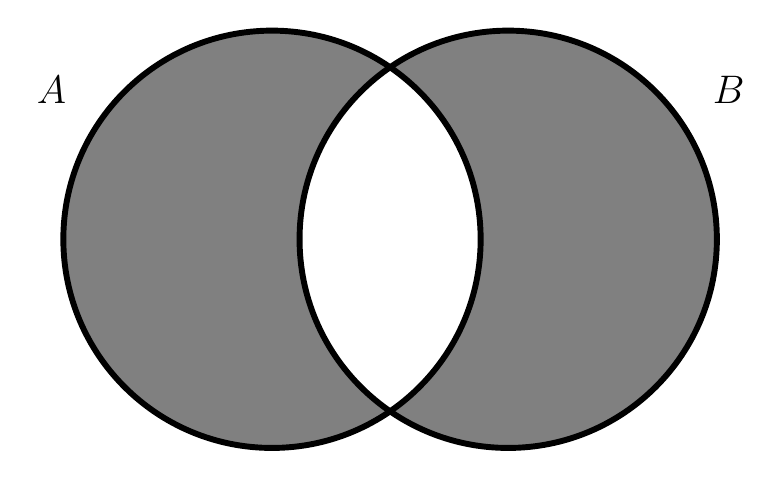
\begin{tikzpicture}
        \def\firstcircle{(-.5,0) circle (2.65cm)}
        \def\secondcircle{(2.5,0) circle (2.65cm)}
        
        % Fill the symmetric difference
        \fill[even odd rule, gray]\firstcircle \secondcircle;
        
        % Draw the circle outlines and add labels
        \draw[draw=black,line width=.75mm] \firstcircle;
        \draw[draw = black, line width=.75mm] \secondcircle;
        \node at (-3.3,1.9) {\Large$A$};
        \node at (5.3,1.9) {\Large$B$};
    \end{tikzpicture}}
    \caption{The gray shaded region represents set symmetric difference $A\bigtriangleup B.$}
    \label{fig:setsim}
\end{figure}



We now describe the continual learning cost $J(\weight(t),\psi(t),\tx(t))$ in the context of definition~\ref{defintersect}.
In particular, the expected value of $J(\weight(t),\psi(t),\tx(t))$ 
is continuous with respect to measure $\mu$ 
if for a small $\varepsilon >0$  we can find a $\delta >0$ such that 
$\abs{J(\weight(t),\psi(t),\tx(t))-J(\weight(t+1),\psi(t+1),\tx(t+1))}<\varepsilon$ for 
all $\tx(t+1)$ such that $\mu(\tx(t)\bigtriangleup \tx(t+1))<\delta.$ 
Thus, if two tasks $\tx(t)$ and $\tx(t+\Delta t)$ are similar 
(i.e. $\mu(\tx(t)\bigtriangleup \tx(t+\Delta t))<\delta)$, 
then the forgetting cost $J$ are similar (i.e. 
$\abs{J(\weight(t),\psi(t),\tx(t))-J(\weight(t+1),\psi(t+1),\tx(t+1))}<\varepsilon$). 
This intuition is formalized in the following theorem, 
where we prove that $J$ is continuous with respect to measure $\mu.$


\begin{theorem}\label{contMeasure}
    Let $(\overline{\tx},\mathcal{B}(\overline{\tx}), \mu)$ be the measure space as 
    defined as in definition~\ref{defintersect}. 
    Assume that the loss function $\ell$ is continuous 
    and bounded across all tasks, that is $\forall t \in [0,T].$ 
    Define $J$ over a task $\tx(\tau)$ as
    \begin{align}
   J(\weight(t),\psi(t),\tx(t)) & = \int_0^t \left( \int_{\vx \in \tx(\tau)} 
       \ell(\fhat(\weight(t),\psi(t))( \vx ) ) \right) \;  d~\tau
    \end{align}
    Then, $ J(\weight(t),\psi(t),\tx(t))$ is continuous with respect to the measure 
    for any $ \tx(t), \tx(t+1) \in \mathcal{B}(\overline{\tx})$ such that 
    $\mu(\tx(t)\bigtriangleup \tx(t+1))<\delta$ $\implies$ 
    $\abs{J(\weight(t+1),\psi(t+1),\tx(t+1))- J(\weight(t),\psi(t),\tx(t))} \leq \epsilon$
\end{theorem}
\begin{proof}
    Suppose that the constant $M_0>0$ bounds $\ell$ on every task. 
    Let $\varepsilon>0$ and  set $\delta = \varepsilon/M_0.$ 
    Further let $A,B \in \mathcal{\mathcal{B}}(\overline{\tx})$ 
    such that $\mu(A\bigtriangleup B)< \delta.$ 
    By disjoint additivity of $\mu$ and triangle inequality assuming that the subinterval $[t, t+\Delta t]$ 
    is divided into exactly one unit such that $\Delta t = 1$ we have
    \begin{align*}
       & \left\vert \int_0^{t+\Delta~t} \left( \int_{\vx \in \tx(\tau)} 
       \ell(\fhat(\weight(t),\psi(t))( \vx ) ) \right) \;  d~\tau - 
       \int_0^t \left( \int_{\vx \in \tx(\tau)} \ell(\fhat(\weight(t),\psi(t))( \vx ) ) \right) \;  d~\tau\right\vert \\
        & = \Big\vert \int_{t}^{t+\Delta t} \left( \int_{\vx \in \tx(\tau)} 
       \ell(\fhat(\weight(t),\psi(t))( \vx ) ) \right) \;  d~\tau \Big\vert\\
        & = \left\vert \int_{\vx \in \tx(t+1)} \ell(\fhat(\weight(t),\psi(t))( \ vx ) )  d\mu 
        - \int_{\vx \in \tx(t)} \ell(\fhat(\weight(t),\psi(t))( \ vx ) ) d\mu \right\vert\\
        & = \Bigg\vert\int_{\tx(t)\setminus \tx(t+1)} \ell(\fhat(\weight(t),\psi(t))( \ vx ) )  d\mu \\
        &+ \int_{\tx(t) \cap \tx(t+1)} \ell(\fhat(\weight(t),\psi(t))( \ vx ) ) d\mu \\
        &- \int_{ \tx(t+1) \setminus  \tx(t)} \ell(\fhat(\weight(t),\psi(t))( \ vx ) ) d\mu \\
        &-\int_{ \tx(t+1) \cap  \tx(t)} \ell(\fhat(\weight(t),\psi(t))( \ vx ) ) d\mu
        \Bigg\vert\\
        & \leq \int_{\tx(t+1) \setminus \tx(t)} \abs{\ell(\fhat(\weight(t),\psi(t))( \ vx ) )} d\mu \\
        &+\int_{\tx(t) \setminus \tx(t+1)}\abs{\ell(\fhat(\weight(t),\psi(t))( \ vx ) )}d\mu.
    \end{align*}
    Then, by the boundedness of $\ell,$
    \begin{align*}
        \int_{\tx(t+1) \setminus \tx(t)} \abs{\ell(\fhat(\weight(t),\psi(t))( \ vx ) )} d\mu
        &+ \int_{\tx(t) \setminus \tx(t+1)} \abs{\ell(\fhat(\weight(t),\psi(t))( \ vx ) )} d\mu \\  
        & \leq M_0\mu(\tx(t) \setminus \tx(t+1)) + M_0\mu(\tx(t+1) \setminus \tx(t)).
    \end{align*}
    Hence,
    \begin{align*}
        M_0\mu(\tx(t) \setminus \tx(t+1)) + M_0\mu(\tx(t+1) \setminus \tx(t)) & = M_0(\mu(\tx(t) \setminus \tx(t+1)) + \mu(\tx(t+1) \setminus \tx(t)))\\
        & = M_0\mu(\tx(t) \bigtriangleup \tx(t+1))\\
        & < M_0 \delta\\
         & = M_0 \frac{\varepsilon}{M_0}\\
         & = \varepsilon.
    \end{align*}
    which gives the result.
\end{proof}

%remark justifying loss bounded on all tasks
\begin{remark}\label{boundedremark}
    It is reasonable to assume this hat there is some c
    onstant $M_0<\infty$ for which $M_i\leq M_0$ 
    for all $i\in \mathbb{N}$ because 
    if one did not exist then the problem would be unsolvable as
    an unbounded loss function would imply that 
    the neural network is not learning anything useful from the data. 
\end{remark}

Theorem \ref{contMeasure} solidifies the notion that similar 
tasks produce similar loss values and the idea that, continuity of 
$J$ is upheld when the tasks are similar. 
In return, this implies that the intersection search space in Figure ~\ref{fig:setsim} and \ref{fig:CL} 
is non-empty. The formal connection of this idea to the intersection space 
and continuity of fogetting cost is proven for the first time in this work. 
Moreover, the contrapositive reveals that dissimilar loss 
values implies dissimilar tasks. However, for an arbitrary CL problem, 
dissimilar tasks may or may not result in dissimilar loss values as this 
depends on the weight training mechanism. This intuition implies that 
if we have two tasks $\tx(t)$ and $\tx(t+\Delta t)$ 
such that $\mu \left( \tx(t)\bigtriangleup \tx(t+\Delta t) \right) \geq \delta$ 
then, we do not know whether $\abs{J(\tx(t))-J(\tx(t+\Delta t))}<\varepsilon$ 
(i.e, similar loss values) or $\abs{J(\tx(t))-J(\tx(t+\Delta t))}\geq\varepsilon$ 
(i.e. dissimilar loss values). 
Nonetheless, it is intuitively clear that, if dissimilar tasks do produce dissimilar loss values, eventually, the intersection space becomes empty
and the continuity of $J$ is violated.
In practice, however, a sudden violation of Theorem \ref{contMeasure} is unlikely to occur. 
Instead, as the number of tasks increase, the value of 
$\abs{J(\tx(t))-J(\tx(t+\Delta t))}$ will tend to increase 
and eventually exceed $\varepsilon.$ Therefore, the model 
will gradually forget prior tasks and eventually CL will fail.  
Where we show that this gradual forgetting
is observed when the architecture is fixed across all tasks.
\KR{reached here with the revision towards making the existence argument more rigorous through 
continuity argument.}

\begin{lemma}\label{lem: taylor}
    Suppose $\tx(t)$ and $\tx(t+1)$ are two consecutive tasks in the measure space $(\overline{\tx}, \mathcal{B}(\overline{\tx}),\mu).$  Set $M_0$ to be the upper bound on the loss function $\ell$ across all tasks and suppose $\psi(t) = \psi(1)$ for all tasks $t.$ Then, for $\mu(\tx(t)\bigtriangleup \tx(t+1))\geq \delta,$ the following holds
    \begin{align*}
        E(\tx(t+\Delta t)) & = E(\tx(t)) + \Delta t\Big[\mu( \tx(t)\Delta \tx(t+\Delta t))\cdot \displaystyle\int_{\tx(t)\Delta \tx(t+\Delta t)} \ell(\hat{f}(\weight,\psi))d\mu\\
        & + \displaystyle\int_{\tx(t)} \ell'(\hat{f}(\weight,\psi))\cdot \partial_{\weight}^1 \hat{f}(\weight,\psi)\cdot \Delta \weight \hspace{1mm}  d\mu\Big]+ o(\Delta t).
    \end{align*}
\end{lemma}

\begin{proof}
    The first-order Taylor series expansion of $E(\tx(t+\Delta t))$ about $t,$ is given by
    \begin{align}
        E(\tx(t+\Delta t)) & = E(\tx(t)) + \Delta t\Big[ E_{\tx} (\tx(t)\Delta \tx(t+\Delta t))+ E_{\weight}(\tx(t))\Big] + o(\Delta t),\label{taylorexp1}
    \end{align}
    where $E_{\tx}$ and $E_{\weight},$ are the partial derivatives of the expected value function with respect to the data and  weights, respectively. Since we assumed $\psi(t) = \psi(1)$ for all $t$ (i.e., the architecture is fixed), note that we did not take the partial derivative of the expected value function with respect to the architecture. 
    
    Now, we work on acquiring each partial derivative. Toward that end, 
    \begin{align}
        E_{\tx} (\tx(t)\Delta \tx(t+\Delta t)) & =\mu( \tx(t)\Delta \tx(t+\Delta t))\cdot \displaystyle\int_{\tx(t)\Delta \tx(t+\Delta t)} \ell(\hat{f}(\weight,\psi))d\mu.\label{E_X1 :thmweight}
    \end{align}
    To determine the remaining two derivatives, we use the Sobolev function chain rule found in \cite{evans2022partial}. We can do so as $\ell$ is real-valued and bounded, and $\ell'$ is continuously differentiable. Then,
    \begin{align}
        E_{\weight} (\tx(t)) & = \displaystyle\int_{\tx(t)} \ell'(\hat{f}(\weight,\psi))\cdot \partial_{\weight}^1 \hat{f}(\weight,\psi)\cdot \Delta w \hspace{1mm}  d\mu.\label{E_w: thmweight}
    \end{align}
    Substituting (\ref{E_X1 :thmweight}) and (\ref{E_w: thmweight})  into the Taylor series expansion (\ref{taylorexp}), we have
    \begin{align*}
        E(\tx(t+\Delta t)) & = E(\tx(t)) + \Delta t\Big[\mu( \tx(t)\Delta \tx(t+\Delta t))\cdot \displaystyle\int_{\tx(t)\Delta \tx(t+\Delta t)} \ell(\hat{f}(\weight,\psi))d\mu\\
        & + \displaystyle\int_{\tx(t)} \ell'(\hat{f}(\weight,\psi))\cdot \partial_{\weight}^1 \hat{f}(\weight,\psi)\cdot \Delta w \hspace{1mm}  d\mu\Big]+ o(\Delta t),
    \end{align*}
    as desired.
\end{proof}
The following theorem is immediate to identify the lower bound on the first difference in the CL cost.
\KR{reached here}

\begin{theorem}
    Suppose $\tx(t)$ and $\tx(t+1)$ are two consecutive tasks in the measure space $(\overline{\tx}, \mathcal{B}(\overline{\tx}),\mu).$ Let $L_1>0$ and $0\leq \delta\leq 1$ all be constants. Set $M_0$ to be the upper bound on the loss function $\ell$ across all tasks. Moreover, suppose $\psi(t) = \psi(1)$ for all tasks $t.$ Then, for $\mu(\tx(t)\bigtriangleup \tx(t+1))\geq \delta,$ the following holds
    \begin{align*}
        E(\tx(T)) - E(\tx(t))
        & \leq \sum_{\tau =t}^{T} \Big( M_0\cdot \delta - \displaystyle\int_{\tx(\tau)} \left(\ell'(\hat{f}(\weight,\psi))\cdot \partial_{\weight}^1 \hat{f}(\weight,\psi)\right)^2 \hspace{1mm}  d\mu \Big)
    \end{align*}
\end{theorem}

\begin{proof}
    To begin, recall that
    \begin{align*}
        J(\weight(t),\psi(t),\tx(t)) & = \int_0^t \left( \int_{\vx \in \tx(\tau)} \ell(\fhat(\weight(t),\psi(t))( \vx ) ) \right) \;  d~\tau\\
        & = \int_0^t E(\tx(\tau))d\tau.
    \end{align*}
    As the expected value function is a continuous, real-valued function on the closed interval $[0,t],$ it follows that
    \begin{align*}
        \nabla J & = \nabla \left( \int_0^t E(\tx(\tau))d\tau\right) = \int_0^t \nabla E(\tx(\tau))d\tau = E(\tx(t)).
    \end{align*}
    By Lemma \ref{lem: taylor} and the previous equation
    \begin{align*}
        \nabla J  &= E(\tx(t)) \\        & = E(\tx(t+\Delta t)) - \Delta t\Big[\mu( \tx(t)\Delta \tx(t+\Delta t))\cdot \displaystyle\int_{\tx(t)\Delta \tx(t+\Delta t)} \ell(\hat{f}(\weight,\psi))d\mu\\
        & +\displaystyle\int_{\tx(t)} \ell'(\hat{f}(\weight,\psi))\cdot \partial_{\weight}^1 \hat{f}(\weight,\psi)\cdot \Delta w \hspace{1mm}  d\mu\Big]- o(\Delta t)\\
        & = E(\tx(t+\Delta t)) + \Delta t(-\mu( \tx(t)\Delta \tx(t+\Delta t)))\cdot \displaystyle\int_{\tx(t)\Delta \tx(t+\Delta t)} \ell(\hat{f}(\weight,\psi))d\mu\\
        & - \Delta t\displaystyle\int_{\tx(t)} \ell'(\hat{f}(\weight,\psi))\cdot \partial_{\weight}^1 \hat{f}(\weight,\psi)\cdot \Delta w \hspace{1mm}  d\mu- o(\Delta t)\\
        & \leq E(\tx(t+\Delta t)) + \Delta t \cdot \delta \cdot \displaystyle\int_{\tx(t)\Delta \tx(t+\Delta t)} \ell(\hat{f}(\weight,\psi))d\mu\\
        & - \Delta t\displaystyle\int_{\tx(t)} \ell'(\hat{f}(\weight,\psi))\cdot \partial_{\weight}^1 \hat{f}(\weight,\psi)\cdot \Delta w \hspace{1mm}  d\mu- o(\Delta t)\\
    \end{align*}
    Subtracting $E(\tx(t+\Delta t))$ from both sides and combining like terms,
    \begin{align*}
         E(\tx(t)) - E(\tx(t+\Delta t))
        & \leq E(\tx(t+\Delta t)) + \Delta t \cdot \delta \cdot \displaystyle\int_{\tx(t)\Delta \tx(t+\Delta t)} \ell(\hat{f}(\weight,\psi))d\mu\\
        & - \Delta t\displaystyle\int_{\tx(t)} \ell'(\hat{f}(\weight,\psi))\cdot \partial_{\weight}^1 \hat{f}(\weight,\psi)\cdot \Delta w \hspace{1mm}  d\mu- o(\Delta t) - E(\tx(t+\Delta t)) \\
        & \leq \Delta t \cdot \delta \cdot \displaystyle\int_{\tx(t)\Delta \tx(t+\Delta t)} \ell(\hat{f}(\weight,\psi))d\mu\\
        & - \Delta t\displaystyle\int_{\tx(t)} \ell'(\hat{f}(\weight,\psi))\cdot \partial_{\weight}^1 \hat{f}(\weight,\psi)\cdot \Delta w \hspace{1mm}  d\mu- o(\Delta t).
    \end{align*}
    Additionally, we can assume that the loss function $\ell$ is bounded above by a constant $M_0,$ so
    \begin{align*}
        E(\tx(t)) - E(\tx(t+\Delta t))
        & \leq \Delta t \cdot \delta M_0
        - \Delta t\displaystyle\int_{\tx(t)} \ell'(\hat{f}(\weight,\psi))\cdot \partial_{\weight}^1 \hat{f}(\weight,\psi)\cdot \Delta w \hspace{1mm}  d\mu- o(\Delta t).
    \end{align*}
    To consider this difference in expected values across future tasks, set $\Delta t =1 $ and let us sum across such future tasks, 
    \begin{align*}
         \sum_{\tau = t}^{T} (E(\tx(\tau)) - E(\tx(\tau+1)))
        & \leq \sum_{\tau =t}^{T} \Big( M_0\cdot \delta - \displaystyle\int_{\tx(\tau)} \ell'(\hat{f}(\weight,\psi))\cdot \partial_{\weight}^1 \hat{f}(\weight,\psi)\cdot \Delta w \hspace{1mm}  d\mu \Big).
    \end{align*}
    Now, we can choose the following for each $\tau$
    \begin{align*}
        \Delta \weight & = \ell'(\hat{f}(\weight,\psi))\cdot \partial_{\weight}^1 \hat{f}(\weight,\psi).
    \end{align*}
    Thus,
    \begin{align*}
         \sum_{\tau = t}^{T} (E(\tx(\tau)) - E(\tx(\tau+1)))
        & \leq \sum_{\tau =t}^{T} \Big( M_0\cdot \delta - \displaystyle\int_{\tx(\tau)} \left(\ell'(\hat{f}(\weight,\psi))\cdot \partial_{\weight}^1 \hat{f}(\weight,\psi)\right)^2 \hspace{1mm}  d\mu \Big),
    \end{align*}
    as desired. Note that the the term $\left(\ell'(\hat{f}(\weight,\psi))\cdot \partial_{\weight}^1 \hat{f}(\weight,\psi)\right)^2$ above is positive, and so the integral will be positive. Thus, we can view the subtraction of this integral as the impact of changing the weights to the overall difference in loss values.
\end{proof}

The lower bound in ( Theorem \ref{lowerw}) confirms that the norm of the gradient is dependent upon the bound on the loss function and the change in the weights. In particular, we see that the more we change the weights $\weight(t),$ the smaller our lower bound gets. As a smaller norm of the gradient implies a smaller change in the expected value between two tasks (i.e. smaller $\abs{E(\tx(t)))-E(\tx(t+\Delta t))}$), it is clear that we could reduce the lower bound in (\ref{lowerw}) by changing the weights. However, we can only change the weights so far before overfitting occurs. In other words, there is a bound on the change in weights, and hence a bound on much we can reduce the lower bound (Theorem \ref{lowerw}). It would be ideal if the lower bound could be reduced further. 

It is important to note that in Theorem \ref{lowerw}, we fix the architecture.  What if we allow for changing the architecture as well? Intuitively, we know changing the architecture via some architecture search will result in a better performing NN (i.e. smaller expected value). However, let us provide a concrete proof to support this intuition. The following theorem provides us with a lower bound on $\|\nabla E\|$ that is smaller than that presented in (\ref{lowerw}). Thus, we have the potential to reduce $\|\nabla E\|$ and hence reduce the change in the expected value $\abs{E(\tx(t)))-E(\tx(t+\Delta t))}.$ 

%theorem for lower bound on weights and architecture
\begin{theorem}\label{lowerpsi}
    Suppose $\tx(t)$ and $\tx(t+1)$ are two consecutive tasks in the measure space $(\overline{\tx}, \mathcal{B}(\overline{\tx}),\mu).$ Let $L_1>0$ and $0\leq \delta\leq 1$ all be constants. Set $M_0$ to be the upperbound on the loss function $\ell$ across all tasks. Then, for $\mu(\tx(t)\bigtriangleup \tx(t+1))\geq \delta,$ the following holds
    \begin{align*}
        \sum_{\tau = t}^{T} (E(\tx(\tau)) - E(\tx(\tau+1)))
        & \leq \sum_{\tau =t}^{T} \Big( M_0\cdot \delta - \displaystyle\int_{\tx(\tau)} \left(\ell'(\hat{f}(\weight,\psi))\cdot \partial_{\weight}^1 \hat{f}(\weight,\psi)\right)^2 \hspace{1mm}  d\mu - \\
        & -\displaystyle\int_{\tx(t)} \left(\ell'(\hat{f}(\weight,\psi))\cdot \partial_\psi^1 \hat{f}(\weight,\psi)\right)^2\hspace{1mm}  d\mu\Big).
    \end{align*}
    
\end{theorem}


\begin{proof}
    To begin, note that the first-order Taylor series expansion of $E(\tx(t+\Delta t))$ about  $t,$ is given by
    \begin{align}
        E(\tx(t+\Delta t)) & = E(\tx(t)) + \Delta t\Big[ E_{\tx} (\tx(t)\Delta \tx(t+\Delta t))+ E_{\weight}(\tx(t)) + E_\psi(\tx(t))\Big] + o(\Delta t),\label{taylorexparch}
    \end{align}
    where $E_{\tx} , E_{\weight},$ and $E_\psi$ are the partial derivatives of the expected value function with respect to the data, weights, and architecture, respectively. Now, we work on acquiring each partial derivative. Toward that end, 
    \begin{align}
        E_{\tx} (\tx(t)\Delta \tx(t+\Delta t)) & =\mu( \tx(t)\Delta \tx(t+\Delta t))\cdot \displaystyle\int_{\tx(t)\Delta \tx(t+\Delta t)} \ell(\hat{f}(\weight,\psi))d\mu.\label{E_X1}
    \end{align}
    To determine the remaining two derivatives, we use the Sobolev function chain rule found in \cite{evans2022partial}. We can do so as $\ell$ is real-valued and bounded, and $\ell'$ is continuously differentiable. Then,
    \begin{align}
        E_{\weight} (\tx(t)) & = \displaystyle\int_{\tx(t)} \ell'(\hat{f}(\weight,\psi))\cdot \partial_{\weight}^1 \hat{f}(\weight,\psi)\cdot \Delta w \hspace{1mm}  d\mu.\label{E_w},\\
        E_\psi (\tx(t)) & = \displaystyle\int_{\tx(t)} \ell'(\hat{f}(\weight,\psi))\cdot \partial_\psi^1 \hat{f}(\weight,\psi)\cdot \Delta \psi \hspace{1mm}  d\mu.\label{E_psi}
    \end{align}
    Substituting (\ref{E_X1}), (\ref{E_w}), and (\ref{E_psi}) into the Taylor series expansion (\ref{taylorexparch}), we have
    \begin{align}
        E(\tx(t+\Delta t)) & = E(\tx(t)) + \Delta t\Big[\mu( \tx(t)\Delta \tx(t+\Delta t))\cdot \displaystyle\int_{\tx(t)\Delta \tx(t+\Delta t)} \ell(\hat{f}(\weight,\psi))d\mu\\
        & + \displaystyle\int_{\tx(t)} \ell'(\hat{f}(\weight,\psi))\cdot \partial_{\weight}^1 \hat{f}(\weight,\psi)\cdot \Delta w \hspace{1mm} d\mu+\displaystyle\int_{\tx(t)} \ell'(\hat{f}(\weight,\psi))\cdot \partial_\psi^1 \hat{f}(\weight,\psi)\cdot \Delta \psi \hspace{1mm}  d\mu\Big]+ o(\Delta t).\label{archfinaltaylor}
    \end{align}
    recall that
    \begin{align*}
        J(\weight(t),\psi(t),\tx(t)) & = \int_0^t \left( \int_{\vx \in \tx(\tau)} \ell(\fhat(\weight(t),\psi(t))( \vx ) ) \right) \;  d~\tau\\
        & = \int_0^t E(\tx(\tau))d\tau.
    \end{align*}
    As the expected value function is a continuous, real-valued function on the closed interval $[0,t],$ it follows that
    \begin{align*}
        \nabla J & = \nabla \left( \int_0^t E(\tx(\tau))d\tau\right) = \int_0^t \nabla E(\tx(\tau))d\tau = E(\tx(t)).
    \end{align*}
    By (\ref{archfinaltaylor}) and the previous equation
    \begin{align*}
       E(\tx(t)) &=  \nabla J \\        & = E(\tx(t+\Delta t)) - \Delta t\Big[\mu( \tx(t)\Delta \tx(t+\Delta t))\cdot \displaystyle\int_{\tx(t)\Delta \tx(t+\Delta t)} \ell(\hat{f}(\weight,\psi))d\mu\\
        & +\displaystyle\int_{\tx(t)} \ell'(\hat{f}(\weight,\psi))\cdot \partial_{\weight}^1 \hat{f}(\weight,\psi)\cdot \Delta w \hspace{1mm}  d\mu + \displaystyle\int_{\tx(t)} \ell'(\hat{f}(\weight,\psi))\cdot \partial_\psi^1 \hat{f}(\weight,\psi)\cdot \Delta \psi \hspace{1mm}  d\mu \Big]- o(\Delta t)\\
        & = E(\tx(t+\Delta t)) + \Delta t(-\mu( \tx(t)\Delta \tx(t+\Delta t)))\cdot \displaystyle\int_{\tx(t)\Delta \tx(t+\Delta t)} \ell(\hat{f}(\weight,\psi))d\mu\\
        & - \Delta t\displaystyle\int_{\tx(t)} \ell'(\hat{f}(\weight,\psi))\cdot \partial_{\weight}^1 \hat{f}(\weight,\psi)\cdot \Delta w \hspace{1mm}  d\mu -\Delta t \displaystyle\int_{\tx(t)} \ell'(\hat{f}(\weight,\psi))\cdot \partial_\psi^1 \hat{f}(\weight,\psi)\cdot \Delta \psi \hspace{1mm}  d\mu- o(\Delta t)\\
        & \leq E(\tx(t+\Delta t)) + \Delta t \cdot \delta \cdot \displaystyle\int_{\tx(t)\Delta \tx(t+\Delta t)} \ell(\hat{f}(\weight,\psi))d\mu\\
        & - \Delta t\displaystyle\int_{\tx(t)} \ell'(\hat{f}(\weight,\psi))\cdot \partial_{\weight}^1 \hat{f}(\weight,\psi)\cdot \Delta w \hspace{1mm}  d\mu- \Delta t \displaystyle\int_{\tx(t)} \ell'(\hat{f}(\weight,\psi))\cdot \partial_\psi^1 \hat{f}(\weight,\psi)\cdot \Delta \psi \hspace{1mm}  d\mu- o(\Delta t).\\
    \end{align*}
    Subtracting $E(\tx(t+\Delta t))$ from both sides and combining like terms,
    \begin{align*}
         E(\tx(t))- E(\tx(t+\Delta t)) &\leq E(\tx(t+\Delta t)) + \Delta t \cdot \delta \cdot \displaystyle\int_{\tx(t)\Delta \tx(t+\Delta t)} \ell(\hat{f}(\weight,\psi))d\mu\\
        & - \Delta t\displaystyle\int_{\tx(t)} \ell'(\hat{f}(\weight,\psi))\cdot \partial_{\weight}^1 \hat{f}(\weight,\psi)\cdot \Delta w \hspace{1mm}  d\mu\\
        & -\Delta t \displaystyle\int_{\tx(t)} \ell'(\hat{f}(\weight,\psi))\cdot \partial_\psi^1 \hat{f}(\weight,\psi)\cdot \Delta \psi \hspace{1mm}  d\mu- o(\Delta t) -E(\tx(t+\Delta t)\\
         & \leq \Delta t \cdot \delta \cdot \displaystyle\int_{\tx(t)\Delta \tx(t+\Delta t)} \ell(\hat{f}(\weight,\psi))d\mu\\
        & - \Delta t\displaystyle\int_{\tx(t)} \ell'(\hat{f}(\weight,\psi))\cdot \partial_{\weight}^1 \hat{f}(\weight,\psi)\cdot \Delta w \hspace{1mm}  d\mu- \Delta t \displaystyle\int_{\tx(t)} \ell'(\hat{f}(\weight,\psi))\cdot \partial_\psi^1 \hat{f}(\weight,\psi)\cdot \Delta \psi \hspace{1mm}  d\mu- o(\Delta t).\\
    \end{align*}

    Additionally, we can assume that the loss function $\ell$ is bounded above by a constant $M_0,$ so
    \begin{align*}
        E(\tx(t)) - E(\tx(t+\Delta t))
        & \leq \Delta t \cdot \delta M_0
        - \Delta t\displaystyle\int_{\tx(t)} \ell'(\hat{f}(\weight,\psi))\cdot \partial_{\weight}^1 \hat{f}(\weight,\psi)\cdot \Delta w \hspace{1mm}  d\mu\\
        & -\Delta t \displaystyle\int_{\tx(t)} \ell'(\hat{f}(\weight,\psi))\cdot \partial_\psi^1 \hat{f}(\weight,\psi)\cdot \Delta \psi \hspace{1mm}  d\mu - o(\Delta t).
    \end{align*}
    To consider this difference in expected values across future tasks, set $\Delta t =1 $ and let us sum across such future tasks, 
    \begin{align*}
         \sum_{\tau = t}^{T} (E(\tx(\tau)) - E(\tx(\tau+1)))
        & \leq \sum_{\tau =t}^{T} \Big( M_0\cdot \delta - \displaystyle\int_{\tx(\tau)} \ell'(\hat{f}(\weight,\psi))\cdot \partial_{\weight}^1 \hat{f}(\weight,\psi)\cdot \Delta w \hspace{1mm}  d\mu \\
        & - \displaystyle\int_{\tx(t)} \ell'(\hat{f}(\weight,\psi))\cdot \partial_\psi^1 \hat{f}(\weight,\psi)\cdot \Delta \psi \hspace{1mm}  d\mu\Big).
    \end{align*}
    Now, we can choose the following for each $\tau$
    \begin{align*}
        \Delta \weight & = \ell'(\hat{f}(\weight,\psi))\cdot \partial_{\weight}^1 \hat{f}(\weight,\psi),
    \end{align*}
    and
    \begin{align*}
        \Delta \psi & = \ell'(\hat{f}(\weight,\psi))\cdot \partial_\psi^1 \hat{f}(\weight,\psi).
    \end{align*}
    Thus,
    \begin{align*}
         \sum_{\tau = t}^{T} (E(\tx(\tau)) - E(\tx(\tau+1)))
        & \leq \sum_{\tau =t}^{T} \Big( M_0\cdot \delta - \displaystyle\int_{\tx(\tau)} \left(\ell'(\hat{f}(\weight,\psi))\cdot \partial_{\weight}^1 \hat{f}(\weight,\psi)\right)^2 \hspace{1mm}  d\mu\\
        & - \displaystyle\int_{\tx(t)} \left(\ell'(\hat{f}(\weight,\psi))\cdot \partial_\psi^1 \hat{f}(\weight,\psi)\right)^2\hspace{1mm}  d\mu\Big),
    \end{align*}
    as desired. Note that the the terms $\left(\ell'(\hat{f}(\weight,\psi))\cdot \partial_{\weight}^1 \hat{f}(\weight,\psi)\right)^2$ and $\left(\ell'(\hat{f}(\weight,\psi))\cdot \partial_\psi^1 \hat{f}(\weight,\psi)\right)^2$ above are positive, and so each respective integral will be positive. Thus, we can view the subtraction of the integral of $\left(\ell'(\hat{f}(\weight,\psi))\cdot \partial_{\weight}^1 \hat{f}(\weight,\psi)\right)^2$ as the impact of changing the weights to the overall difference in loss values, and the subtraction of the integral of $\left(\ell'(\hat{f}(\weight,\psi))\cdot \partial_\psi^1 \hat{f}(\weight,\psi)\right)^2$ as the impact of changing the architecture to the overall difference in loss values.
\end{proof}

The previous theorem provided us with a lower bound (\ref{lowerpsi}) which was inherently smaller than (\ref{lowerw}) since we now can subtract the change in the architecture $\psi(t)$ as well as the change in the weights $\weight(t).$  This leads us to the following corollary.

\begin{corollary}\label{archCor}
    Suppose $\tx(t)$ and $\tx(t+\Delta t)$ are two consecutive tasks in the measure space $(\overline{\tx}, \mathcal{B}(\overline{\tx}), \mu).$ Let $\mu(\tx(t)\bigtriangleup \tx(t+\Delta t))\geq \delta$ for $0<\delta \leq 1.$ The architecture $\psi$ of a network can be changed to absorb the impact of $\mu(\tx(t)\bigtriangleup \tx(t+\Delta t))\geq \delta.$
\end{corollary}

\begin{proof}
Let $\varepsilon >0$ small. Since the expected value function is continuous with respect to measure by Theorem \ref{contMeasure}, we can find a corresponding $\delta>0.$ Suppose we have two tasks $\tx(t)$ and $\tx(t+\Delta t))$ for which $\mu(\tx(t)\bigtriangleup \tx(t+\Delta t))\geq \delta.$ Moreover, suppose $\abs{E(\tx(t+\Delta t))-E(\tx(t))}\geq \varepsilon.$ Then, by Theorem \ref{lowerpsi}, we see that changing the architecture and training on a new optimal architecture that we can have
    \begin{align}  
    \abs{\nabla E(\tx(t))}& \geq M_0\delta - L_1\abs{\Delta w}\displaystyle\int_{\tx(t)} \|\partial^1_{\weight} \hat{f}(w(t,\psi),\psi(t))\|_{L^p}d\mu - L_1\abs{\Delta \psi}\displaystyle\int_{\tx(t)} \|\partial^1_\psi \hat{f}(w(t,\psi),\psi(t))\|_{L^p}d\mu. 
    \label{eq:final}
    \end{align}
Thus, changing the architecture of the network can offset the impact of consecutive tasks whose data differ substantially.
\end{proof}
\KR{I am going to go from here and build the rest of the paper, we will revise the above when you get a chance to fix the theorem.}

Due to Corollary \ref{archCor}, the intersection space that offers feasible solutions to the continual learning problem vanishes as the data distribution changes over time. As a consequence, it is then necessary to change the architecture so as to increase the potential size of the intersection space. In particular, we do not fix the architecture for our problem.


\begin{figure}
    \centering
    \includegraphics[width=\linewidth]{paperFigures/intersect22.png}
    \caption{The Solution, where we change the size of the intersection space by introducing more capacity, through choosing novel hyperparameters}
    \label{fig:solution}
\end{figure}
To understand how this can be accomplished, consider Figure  \ref{fig:solution}, which describes the method for the first and second task. We begin at task $t = 1$ and determine an optimal weight denoted $w^*(1) = w^\infty(1).$ This gives us a NN solution in $\mathcal{F}_1.$ Then, as the next task is observed, we perform a derivative free hyper-parameter search, in particular, the directional direct search method~\cite{larson2019derivative} to obtain new architecture. The solution to this search is denoted $\psi^\infty(2)$ as in  Figure ~\ref{fig:solution}

Notably, there is a new quandary, since the new architecture introduces a parameter space that may be of different size than the one used for the previous task, it is unfortunately not feasible to trivially transfer information from the previous architecture to the new one. The common and the state of the art solution to this problem is to initialize the parameters in the new architecture from random and retrain on all available tasks, which is resource heavy as well as impractical. To obviate this necessity, we develop a low rank transfer algorithm that seeks to transfer information between the previous architecture to the new architecture in an efficient way. We describe this solution next.


\section{CL Solution}
In particulaer, our goal is to solve the following bilevel problem
\begin{align}\label{eq:bilevel} \tag{bi-level}
     V^*(t,\weight(t))  = \min_{\weight \in \mathcal{W}(\psi^*(t))} V(t,\weight(t)),\quad \text{ where}\; \;  \psi^*(t)  = \mathrm{arg}\min_{\psi\in \Psi} J(\weight(t),\psi,\tx(t)),
\end{align}
Noting that the weight search space at each $t$ is a function of the optimal architecture, we change the weight space for each $t$ as 
\begin{align}
    \weight(t+\Delta~t) = \mathrm{A}^* (t) \weight(t) \mathrm{B}(t)^*T,
\end{align}
where $\mathrm{A}$ and $\mathrm{B}$ are matrices that enable the transfer of information between two different parameter space and $\mathrm{A}^*, \mathrm{B}^*$ ar the optimal values such that loss of information is minimal. This change in the weight space for each new task introduce dynamics into the continual learning problem defined by $V^*.$ The following result therefore provides the total variation in $V^*$ as a function of tasks.
\begin{proposition}\label{HJB}
    The total variation in $V^*(t)$ at any given task $t$ is given by
    \begin{align}\label{eq:HJB}
        -\frac{\partial V^*}{\partial t}& = \min_{\weight \in \mathcal{W}(\psi^*(t))} J(\weight(t),\psi^*(t),\tx(t)) + \frac{\partial V^*}{\partial \tx}\frac{d\tx}{dt}+ \frac{\partial V^*}{\partial \weight}[\mathrm{A}^*(t)\weight(t)( \mathrm{B}^*(t))^T + u(t)],
    \end{align}
    where $\mathrm{A}^*(t),B^*(t)$ are optimal $\mathrm{A}(t)$ and $\mathrm{B}(t)$ for task $t$ and $u(t)$ represents the updates made to the each weights matrix of the new dimensions. 
\end{proposition}
\begin{proof}[proof of Proposition \ref{HJB}]
    Let $J, V,$ and $V^*$ be as defined above. To begin, we split the sum in $V(t)$ over the discrete intervals $[t,t+\Delta t]$ and $[t+\Delta t, T].$ Observe,
    \begin{align}\label{b}
        V^*(t) & = \min_{w\in \mathcal{W}(\psi^*(t))} \int_{t}^T J(w(\tau),\psi^*(t), \tx(\tau))d\tau\nonumber\\
                & = \min_{w\in \mathcal{W}(\psi^*(t))} \biggr[\int_{t}^{t+\Delta t} J(w(\tau),\psi^*(t), \tx(\tau))d\tau+ \int_{t+\Delta t}^{T} J(w(\tau),\psi^*(t), \tx(\tau))d\tau\biggr]\nonumber\\
                & = \min_{w\in \mathcal{W}(\psi^*(t))} \int_{t}^{t+\Delta t} J(w(\tau),\psi^*(t),\tx(\tau))d\tau + V^*(t+\Delta t)\nonumber\\
                & = \min_{w\in \mathcal{W}(\psi^*(t))} J(\weight(t),\psi^*(t),\tx(t))\Delta t + V^*(t+\Delta t).
    \end{align}
    Now, we provide the Taylor series expansion of $V^*(t+\Delta t)$ about $t.$ Notice,
    \begin{align}
        V^*(t+\Delta t) & = V^*(t) + \Delta t \left[\frac{\partial V^*}{\partial t} + \frac{\partial V^*}{\partial \tx}\frac{d\tx}{dt} + \frac{\partial V^*}{\partial \weight}\frac{\partial \weight}{dt}\right] + o(\Delta t)\nonumber\\
                & = V^*(t) + \Delta t\biggr[\frac{\partial V^*}{\partial t} + \frac{\partial V^*}{\partial \tx}\frac{d\tx}{dt} + \frac{\partial V^*}{\partial \weight}[\mathrm{A}^*(t)\weight(t)( \mathrm{B}^*(t))^T + u(t)]\biggr] + o(\Delta t),\label{a}
    \end{align}
    where $u(t)$ represents the updates made to the each weights matrix of the new dimensions.
    Substituting \ref{a} into \ref{b}, we have
    \begin{align*}
        V^*(t) & = \min_{w\in \mathcal{W}(\psi^*(t))} J(\weight(t),\psi^*(t),\tx(t))\Delta t+ V^*(t) + \Delta t\biggr[\frac{\partial V^*}{\partial t} + \frac{\partial V^*}{\partial \tx}\frac{d\tx}{dt} + \frac{\partial V^*}{\partial \weight}[\mathrm{A}^*(t)\weight(t)( \mathrm{B}^*(t))^T + u(t)]\biggr] + o(\Delta t).
    \end{align*}
    Canceling $V^*(t)$ gives
    \begin{align*}
        0 & = \min_{w\in \mathcal{W}(\psi^*(t))} J(\weight(t),\psi^*(t),\tx(t))\Delta t+ \Delta t\left[\frac{\partial V^*}{\partial t} + \frac{\partial V^*}{\partial \tx}\frac{d\tx}{dt}+ \frac{\partial V^*}{\partial \weight}[\mathrm{A}^*(t)\weight(t)( \mathrm{B}^*(t))^T + u(t)]\right] + o(\Delta t).
    \end{align*}
    Dividing both sides by $\Delta t$ produces
    \begin{align*}
        0 & = \min_{w\in \mathcal{W}(\psi^*(t))} J(\weight(t),\psi^*(t),\tx(t)) +
        \frac{\partial V^*}{\partial t} + \frac{\partial V^*}{\partial \tx}\frac{d\tx}{dt} + \frac{\partial V^*}{\partial \weight}[\mathrm{A}^*(t)\weight(t)( \mathrm{B}^*(t))^T + u(t)].
    \end{align*}
    Finally, reordering gives
    \begin{align*}
        -\frac{\partial V^*}{\partial t} & = \min_{w\in \mathcal{W}(\psi^*(t))} J(\weight(t),\psi^*(t),\tx(t))+ \frac{\partial V^*}{\partial \tx}\frac{d\tx}{dt} + \frac{\partial V^*}{\partial \weight}[\mathrm{A}^*(t)\weight(t)( \mathrm{B}^*(t))^T + u(t)],
    \end{align*}
    as desired.
\end{proof}
Observe that \eqref{eq:HJB} is missing the term $\frac{\partial V^*}{\partial \psi}\frac{\partial \psi}{\partial t},$ this is intentional as the exact effects of architecture cannot be measured through derivatives in this PDE. Instead, in this PDE, this effect is absorbed through the change in tensors $\mathrm{A}(t)$ and $\mathrm{B}(t)$. Due to this absorption, it is feasible to now define a lower bound on the first different as follows.
\begin{theorem}\label{thm:lower_HJB}
Given proposition~\ref{HJB}, assume there exists an stochastic gradient based optimization procedure  and choose $ u(t) =- \sum^{I} \alpha(i) \mathrm{g}^{(i)},$ where $I$ is the number of updates and $\alpha(i)$ is some learning rate. Choose $\alpha(i)$ such that $\norm{\mathrm{g}_{\mathrm{MIN} }}  \norm{\sum^{I} \alpha(i) } \rightarrow 0$ as $I \rightarrow \infty$ and $\min_{\weight \in \mathcal{W}(\psi^*(t))} J(\weight(t),\psi^*(t),\tx(t)) \leq \epsilon.$ Then, as long as the architecture is chosen such that $\singw \norm{\mathrm{A}^*(t)\weight(t)( \mathrm{B}^*(t))^T} = \sing \delta,$ the total variance in the continual learning problem due to the data is bounded by $\epsilon.$
\end{theorem}
\begin{proof}
Given proposition~\ref{HJB}, assume there exists an stochastic gradient based optimization procedure  and choose $ u(t) =- \sum^{I} \alpha(i) \mathrm{g}^{(i)}$  such that $\min_{\weight \in \mathcal{W}(\psi^*(t))} J(\weight(t),\psi^*(t),\tx(t)) \leq \epsilon,$ where $I$ is the number of updates. Then, we have 
\begin{align*}
    -\frac{\partial V^*}{\partial t} & \leq \epsilon + \frac{\partial V^*}{\partial \tx}\frac{d\tx}{dt} +  \frac{\partial V^*}{\partial \weight} \left( \mathrm{A}^*(t)\weight(t)( \mathrm{B}^*(t))^T - \sum^{I} \alpha(i) \mathrm{g}^{(i)}  \right)  \\    
\end{align*}
For any $dt$ in terms of tasks $t$  let $\frac{\partial V^*}{\partial \tx}\frac{d\tx}{dt} \leq \norm{\frac{\partial V^*}{\partial \tx}} \norm{\frac{d\tx}{dt}} \leq \sing \delta$ as $\norm{\frac{d\tx}{dt}}  \geq \mu(\tx(t)\bigtriangleup \tx(t+1)) \geq \delta$ and $\norm{\frac{\partial V^*}{\partial \tx}}$ is less than the largest singular value of $\frac{\partial V^*}{\partial \tx}.$  Thus we write 
\begin{align*}
    -\frac{\partial V^*}{\partial t} & \leq \epsilon + \sing \delta +  \frac{\partial V^*}{\partial \weight} \left( \mathrm{A}^*(t)\weight(t)( \mathrm{B}^*(t))^T - \sum^{I} \alpha(i) \mathrm{g}^{(i)}  \right) 
\end{align*}
Taking $g_{MIN}$ to be the smallest value of the gradient over all update iterations, we have 
\begin{align*}
    -\frac{\partial V^*}{\partial t} & \leq \epsilon + \sing \delta +  \frac{\partial V^*}{\partial \weight} \left( \mathrm{A}^*(t)\weight(t) (\mathrm{B}^*(t))^T - \mathrm{g}_{\mathrm{MIN} } \sum^{I} \alpha(i)  \right) \\
     & \leq \epsilon + \sing \delta +  \norm{\frac{\partial V^*}{\partial \weight}} \norm{\mathrm{A}^*(t)\weight(t)( \mathrm{B}^*(t))^T} - \frac{\partial V^*}{\partial \weight} \left(  \mathrm{g}_{\mathrm{MIN} } \sum^{I} \alpha(i)  \right) \\
     & \leq \epsilon + \left[\sing \delta +  \singw \norm{\mathrm{A}^*(t)\weight(t)( \mathrm{B}^*(t))^T} - \singmin \norm{\mathrm{g}_{\mathrm{MIN} }} \norm{\sum^{I} \alpha(i) } \right]
\end{align*}
This finally provides 
\begin{align*}
    \frac{\partial V^*}{\partial t} & \leq \mathrm{MAX} \epsilon - \mathrm{MIN} \left[\sing \delta +  \singw \norm{\mathrm{A}^*(t)\weight(t)( \mathrm{B}^*(t))^T} - \singmin \norm{\mathrm{g}_{\mathrm{MIN} }} \norm{\sum^{I} \alpha(i) } \right]
\end{align*}
For the total variation to be upper bounded, we need the quantity in the brackets to go to zero, this provides.
\begin{align*}
\left[\sing \delta +  \singw \norm{\mathrm{A}^*(t)\weight(t)( \mathrm{B}^*(t))^T} - \singmin \norm{\mathrm{g}_{\mathrm{MIN} }} \norm{\sum^{I} \alpha(i) } \right] = 0 \\
\end{align*}
\begin{align*}
   \sing \delta &= \left[ \singmin \norm{\mathrm{g}_{\mathrm{MIN} }}  \norm{\sum^{I} \alpha(i) } - \singw \norm{\mathrm{A}^*(t)\weight(t)( \mathrm{B}^*(t))^T} \right]
\end{align*}
Therefore, even when $\alpha(i)$ is chosen such that $\norm{\mathrm{g}_{\mathrm{MIN} }}  \norm{\sum^{I} \alpha(i) } $ as $I \rightarrow \infty,$ $\sing \delta$ can be countered by 
$\singw \norm{\mathrm{A}^*(t)\weight(t)( \mathrm{B}^*(t))^T}$ and this bound is tunable due to the change in the architecture. Therefore, as long as $\singw \norm{\mathrm{A}^*(t)\weight(t)( \mathrm{B}^*(t))^T} = \sing \delta$ the total variance is bounded for all t.
\end{proof}
\begin{remark}
    Theorem~\ref{thm:lower_HJB} is crucial because, it shows that, in the presence of a perfect stochastic gradient algorithm, the change in the tasks can be countered by the choice of the architecture. By choosing a new architecture and introducing the $A$ and $B$ matrices such that, within the CL problem, the effect of varying data distribution can be mitigated and the CL problem can be acceptably solved.
\end{remark}
Therefore, the rest of the section is dedicated to constructing an algorithm such that the condition to ensure convergence is satisfied. In summary~(refer Figure~\ref{fig:method}), for every new task, we utilize an off the shelf algorithm to search for a new optimal architecture. Once a new architecture is found,  we complete what we call ``Low Rank Transfer" from previous task's optimal weights to the new task parameter space. Then, using an off the shelf continual learning algorithm, we train the new architecture for the new task while balancing memory on all the prior tasks.  In the process of Low Rank Transfer, we guarantee transfer of learning by requiring that the $\frac{\partial V^*}{\partial t} \leq \eta$, allowing for the intersection of the NN search spaces between subsequent tasks to increase. Thus, there are three components in our algorithm, step 1: the architecture search, step 2: the low rank transfer and step 3: the continual learning. While step 3 is directly adapted from \cite{chakraborty2025understanding, raghavan2021formalizing}, step 1 and 2 are novel contributions for this work.
\begin{figure}
    \centering
    \includegraphics[width=1.1\linewidth]{paperFigures/method.png}
    \caption{How we do this?}
    \label{fig:method}
\end{figure}


\subsection{\underline{Step 1:}  Architecture Search}\label{archsearch}

Although there are numerous architecture search methods that we could employ, we chose a derivative-free approach that completes a local search using finite difference approximations. This choice was made to mimic the weak derivatives available to us from viewing NN as functions of Sobolev spaces. It will become evident in section \ref{HJB} that a notion of the change in the architecture is needed in order to model the dynamics and solve the lower optimization. We call the search method used a neighborhood directional direct-search (NDDS). The standard directional direct-search method is described in the survey by \cite{larson2019derivative}. 


The intuition behind NDDS is that we check ``neighboring" architectures and compare the expected value of the NN when it trains on the neighboring architecture to that of the current architecture. If the neighboring architecture has a smaller expected value, then we ``move" in that direction by selecting it as the new architecture. We then check the ``neighbors" of this new architecture. As the architecture is a discrete variable, this search method provides a notion of a ``gradient." 

With this intuition, we now describe NDDS in depth. As we discuss this method, consult Algorithm \ref{DDSalg}. For task $t\in \tT,$ set $\tx = \mathcal{Y}$ to be our training data and $J(\weight(t),\psi(t), \mathcal{Y})$ the expected value function. Set $x_s = \psi(t)$ and let $D_s$ be a finite set of directions. Further, we choose a ``step size" $\alpha_s\in \mathbb{N}.$ Now we generate the ``neighboring" points for $x_s$ via $D_s$ and $\alpha_s.$ We call these points \textit{poll points} and define them below
\begin{align*}
    Poll Points = \{x_s + \alpha_s d_i:d_i\in D_s\}.
\end{align*}
Now, using a randomly selected subset of our data, denoted $\mathcal{Y}_s,$ we determine and compare the expected value of NN with randomly initialize weights according to each poll point architecture. If one of these poll points results in a smaller expected value than $x_s,$ we set $x_s$ equal to the poll point. We then repeat this process starting with this new architecture. This search terminates when the expected value is beneath a previously chosen threshold or after five times of repeating. In practice, we chose the threshold to be a percentage lower than the expected value produced by the original architecture.
\KR{Wasnt there a nice diagram you had to illustrate this?}

Let us walk through an example. Suppose we would like to learn the optimal number of neurons per layer in our hidden layers for training a feedforward neural network (FNN) on a data set. Due to the data, suppose the input layer is fixed at $784$ neurons and the output layer is fixed at $10$ neurons per layer. Let us fix the number of hidden layers at $2$ begin with $50$ neurons in each hidden layer. We set $\mathcal{Y}_s$  to be a randomly chosen appropriately sized subset of task $t$ data and previous task data. Our direction set is $D_s = D = \{[0,0,10,0],[0,10,0,0]\}$ and will be the same for every $s.$ For our search, we start by setting the step size $\alpha_s = 10.$ For the first round, we have $x_s = [784,50,50,10],$ so our poll points are $[784,60,50,10],[784,50,60,10],$ and $[784,60,60,10].$ We then train a FNN of each size on the data set $Y_s$ and determine the corresponding expected values. If the expected value of the FNN $[784,60,50,10]$ is smaller than that of the FNN $[784,50,50,10],$ for example, then $x_s = [784,60,50,10].$ We would then continue this process until the expected value of our network is less than our set threshold or we exhaust our neighborhood search. 


% \begin{algorithm}\label{DDSalg}
% \caption{Neighborhood Direct-Directional Search (NDDS)}
% Choose architecture initial point $x_s,$ and step size $\alpha_0\in \mathbb{N}$\\
% Set step parameters
% $\mathrm{threshold}\in \mathbb{R}$\\
% j = 0\\
%  loss $\gets \texttt{training\_loop}(x_s,Y_s)$\\
%  \While{$\mathrm{loss}>\mathrm{threshold}$ or $j<5$}
%     {pollPoints = $\{x_s+\alpha_sd_i:d_i\in D_s\}$\\
%         \For{ $\mathrm{poll\, in\, pollPoints}$}{
%         loss_s $\gets$ \texttt{training\_loop} $(\mathrm{poll},\mathcal{Y}_s)$\\
%       \eIf{$\mathrm{loss}\leq \mathrm{loss}_s$}{
%        $x_{s} = x_s$\;
%        }{
%        $x_{s} = \mathrm{poll}$\;
%        $\mathrm{loss} = \mathrm{loss}_s$\\
%       }
      
%       } $j= j+1;$ }
% \end{algorithm}

\begin{algorithm}[t]
\caption{Neighborhood Direct-Directional Search (NDDS)} \label{DDSalg}
\KwIn{Initial architecture $x_s$, step size $\alpha_0 \in \mathbb{N}$}
\KwIn{Threshold parameter $\mathrm{threshold} \in \mathbb{R}$}
\KwOut{Updated architecture $x_s$}

$j \gets 0$\;
$\mathrm{loss} \gets \texttt{training\_loop}(x_s, \mathcal{Y}_s)$\;
\While{$\mathrm{loss} > \mathrm{threshold}$ \textbf{or} $j < 5$}{
    $\mathrm{pollPoints} \gets \{x_s + \alpha_s d_i : d_i \in D_s\}$\;
    \ForEach{$\mathrm{poll} \in \mathrm{pollPoints}$}{
        $\mathrm{loss}_s \gets \texttt{training\_loop}(\mathrm{poll}, \mathcal{Y}_s)$\;
        \eIf{$\mathrm{loss} \leq \mathrm{loss}_s$}{
            $x_s \gets x_s$\;
        }{
            $x_s \gets \mathrm{poll}$\;
            $\mathrm{loss} \gets \mathrm{loss}_s$\;
        }
    }
    $j \gets j + 1$\;
}
\end{algorithm}



\subsection{\underline{Step 2:}  Low Rank Transfer}\label{LRTsec}

Now that the optimal architecture (i.e. number of neurons per layer) has been determined for the current task, it is immediately obvious that that the size of the weights tensor will not match with the new architecture. Thus, we seek a method to determine a weights tensor corresponding to the new optimal architecture that retains previously learned information and transfers it. We propose a method we call Low Rank Transfer. 

Before we dive into the steps of this method, let us set some assumptions and notation. Recall that the only component of the architecture we seek to learn is the number of neurons per layer in our neural network. Thus, we assume our network has $d$ layers, and we fix all other architecture parameters except for the number of neurons in our hidden layers. From our Definition \ref{defn:NN},  $\psi_i(t)$  provides the dimensions for the corresponding weights matrix in each layer of our network.

In order of appearance, we assign the values of $\psi(t)$ to the values $r_i,s_i$ for each $i$ such that $1\leq i\leq d.$ If $\psi^*(t)$ represents the optimal architecture returned from the NDDS completed for task $t,$ then similarly we can assign the values of the dimensions of the weights matrices of each layer of $\psi_i^*(t)$ to be $a_i,b_i$ for $1\leq i\leq d.$ Our goal is to utilizing the original weights matrices to project into the weights matrix space for the new architecture.

To begin, we initialize dimension $3$ tensors $\mathrm{A}(t),\mathrm{B}(t),$ which are each comprised of $d$ matrices. Let each matrix $\mathrm{A}_i(t)$ in $\mathrm{A}(t)$ be randomly generated with dimensions $a_i\times r_i$ for $1\leq i\leq d.$ Similarly, let each matrix $\mathrm{B}_i $ in $\mathrm{B}(t)$ be randomly generated with size $b_i\times s_i$ for $1\leq i\leq d.$ Then, set $C(t) = \mathrm{A}(t)\weight(t)\mathrm{B}^T(t).$ More specifically $C(t)$ is comprised of $d$ matrices such that $C_i(t) = \mathrm{A}_i(t)\weight_i(t)B^T_i(t)$ for all $1\leq i\leq d.$ Notice, that the dimensions of each $C_i(t)$ are $a_i\times b_i.$ These are the dimensions of the weights matrices for a NN with the new optimal architecture $\psi^*(t).$ See Figure \ref{LRT} to understand the construction of $C(t)$ more explicitly.
    \begin{figure}
        \centering
        \includegraphics[width=\linewidth]{paperFigures/CLsolution1.png}
        \caption{Method of Low Rank Transfer at a single layer} \label{LRT}
    \end{figure}

 To prevent loss of information from $\weight(t),$ when we make the transfer to $C(t),$ we shall train only the $\mathrm{A}(t)$ and $\mathrm{B}(t)$ portions of the new weights tensor $C(t)$ on the task data for a chosen number of epochs, while freezing the $\weight(t)$ tensor. This additional training ensures a transfer of learning to the new weights corresponding to the new optimal architecture. If $C^*(t)$ represents $C(t)$ after this training on just tensors $\mathrm{A}(t)$ and $\mathrm{B}(t)$ and $\psi(t+1) = \psi^*(t),$ then we conclude our process by letting $w(t+1) = C^*(t)$ and completing the standard training of our neural network $\hat{f}(w(t+1),\psi(t+1)$ on task data. 
 
 In algorithm \ref{alg:three}, we summarize each step of our method described in the previous subsections.
 
\begin{algorithm}
\caption{Main Training Loop}\label{alg:three}
Choose $\weight(t)$ and $\psi(t)$ to begin\\
Set \texttt{epoch hyper-parameter}\\
\For{$t = 0,1,\ldots, T$}{
 \textbf{Step 1:} Standard Training of $\weight(t)$\\
    $\weight(t) \gets $\texttt{training\_loop}($\weight(t),\psi(t),$ $\tx(t)$, \texttt{epochs})\\

 \textbf{Step 2:} Architecture Search\\
    $\psi^*(t) \gets$ \texttt{NDDS}$(\psi(t),$ $\tx(t)$)\\
    
\textbf{Step 3:} Initialize $\mathrm{A}(t), \mathrm{B}(t)$\\
\For{$i = 1,...,d$}{
    $\mathrm{A}_i(t), \mathrm{B}_i  \gets$\texttt{init\_AB}($a_i,b_i,r_i,s_i)$}

 \textbf{Step 4:} Set $C(t)$\\
    \For{$i = 1,...,d$}{$C_i(t) = \mathrm{A}_i(t)\weight_i(t)B_i^T(t)$}

 \textbf{Step 5:} Fix $\weight(t),$ Train $\mathrm{A}(t),\mathrm{B}(t)$ for $\hat{f}(C(t),\psi(t+1))$\\
    $C^*(t) \gets$ \texttt{train\_AB}($C(t), \psi(t+1),$ $\tx(t)$, \texttt{epochs})\\

 \textbf{Step 6:} Set New Weights and Architecture\\
    $w(t+1) = C^*(t)$\\
    $\psi(t+1) = \psi^*(t)$\\

 \textbf{Step 7:} Standard Training on New NN
    \texttt{training\_loop}\\($\weight(t+1),\psi(t+1),$ $\tx(t)$, \texttt{epochs})
}
\end{algorithm}
\KR{reached here}

\section{Related Works}
As noted in the introduction, theoretical and empirical results have proven that even in traditional machine learning, training weights of the network alone is not enough. By utilizing tools such as NAS (Neural Architecture Search), LoRA (Low-Rank Adaptation), and PEFT (Parameter-Efficient Fine Tuning), the accuracy of a trained model can readily be increased (\cite{liu2021survey}, \cite{LORAhu2022lora}, and \cite{han2024parameter}). However, in the context of CL, learning optimal hyperparameters or architecture for each task poses a challenge. Not only is it necessary to determine what the optimal hyperparameters are at each task, but it is imperative that learning of previous tasks is transferred.

Toward this end, networks with dynamic structures, such as Progressive Neural Networks (PGN)  and Dynamically Expandable Networks (DEN) were introduced in \cite{rusu2016progressive} and \cite{yoon2017lifelong}. Progressive Neural Networks add a layer to the neural network at each observed task \cite{rusu2016progressive}. While the model's accuracy did improve with such structure, extensive compute time is unavoidable as more tasks, and hence layers, are observed. Dynamically Expandable Networks attempted to remedy the computing issues of PGNs. DENs first determine a sub-collection of neurons to train on for a given task (via a metric) and then add a layer of neurons to the network where appropriate \cite{yoon2017lifelong}. This method also completes sparse regularization at each task to prune the network in attempt to reduce compute time compared to PGNs. The use of a DEN did improve the model's accuracy. However, drawbacks such as compute time, overfitting, and transfer of learning still remained. Learning from previous tasks was not fully transferred, as the weights corresponding to the newly added network layers were randomly initialized. 

In more recent years, researchers have built upon the idea of DENs by developing methods which optimally choose how and when to adjust network architecture. CLEAS (Continual Learning with Efficient Architecture Search) is the first integration of NAS into the CL framework \cite{CLEASgao2022CLEAS}. This method only changes architecture when deemed necessary by utilizing a neuron-level NAS, rather than adding an entire layer to the neural network. Moreover, they prune their network at each step to remove unnecessary layers and/or neurons. The algorithm touts its smaller, purposely learned network structure, as it allows for reduced network complexity, and hence computation time. In particular, CLEAS improves model accuracy by up to $6.70\%$ and reduced network complexity by up to $51.0\%$ on the three benchmark datasets. A strategy similar to CLEAS is CAS (Continual Architecture Search) by \cite{CASpasunuru2019continual}. The premise of only adding and removing to the architecture when deemed optimal for a given task, remains the same. However, rather than using NAS, they use what they call Efficient Neural Architecture Search (ENAS), which incorporates a weight-sharing strategy. SEAL (Searching Expandable Architectures for Incremental Learning) again seeks to change only the hyperparameters and architecture of the NN when necessary, but the method differs from CLEAS in how it determines when to alter the network \cite{SEALgambella2025SEAL}. In particular, SEAL uses a capacity estimation metric to make such decision.

The previous methods all sought to expand the network in some fashion to increase the accuracy of the network. Now, we shift to how parameter-efficient fine-tuning methods have been utilized in CL. In particular, we investigate the use of LoRA (Low-Rank Adaptation) \cite{LORAhu2022lora}. The two methods we will discuss here are intended for pre-trained transformers which are now attempting to learn tasks. The CoLoRA method utilizes a new LoRA adapter for each new task to train a task expert model \cite{wistuba2023continual}. The expert model is then used to train the transformer. At the time, this method produced state of the art results, but it maintains a high computational cost. Since then, the CLoRA method has been introduced \cite{CLORAmuralidhara2025}. The key difference between these two strategies is the number of LoRA adapters. Rather than reinitializing and training a new LoRA adapter for each task, they use a single-adapter approach. This reduces the compute time, while maintaining accuracy and transferring learning.

In this paper, we attempt to combine the most profitable aspects of methods like CLEAS and CLoRA. In other words, our goal is to learn the optimal architecture for each task and utilize a low-rank transfer method to optimally transfer learning to the new architecture. The use of a LoRA-like method to easily guarentee transfer of learning from one architecture to another in standard CL has not been accomplished. Moreover, no previous algorithm has provided a theoretical mathematics framework to support their empirical data. 



\section{Experimental Results}
In this section, we evaluate the algorithm presented above for regression, classification, and graph classification continual learning problems. For all three learning problems, we compare the performance of our algorithm to the standard continual learning approach utilized in \cite{raghavan2021formalizing}. For the regression problem, we consider the randomly generated sine data set and complete experiments where we learn five and $10$ tasks. For the classification problem, we consider the Omniglot data set, which consists of handwritten characters. We also complete experiments where we learn five tasks in this setting. For the graph classification problem, we consider a set of randomly generated images utilizing the FakeDataset from PyTorch and complete experiments where we learn five tasks.


\subsection{Regression}
For the regression problem, we will complete three experiments. In each experiment, we use a feedforward neural network with four layers where we begin with $75$ neurons in each of the hidden layers. We use AdamW with a learning rate of $1\times 10^{-4}$ in the training regime.

In the first experiment, we learn five tasks and train $500$ epochs on each task. Figure \ref{reg5taskstrain} reveals the loss values as the NN trains (on the training data) with respect to different methods on the five tasks. The red graph is the standard continual learning method used in \cite{raghavan2021formalizing}, where no change is made to the architecture across tasks. This serves as our baseline for comparison. The blue graph describes the loss value if we change the architecture at each task, but rather than utilizing the low rank transfer method we describe in \ref{alg:three}, we randomly reinitialize the weights. The green graph shows the loss value when our method of changing the architecture at each step and completing the low rank transfer to retain learning.

The blue graph suggests that changing architecture without transfer of learning leads to loss of learning. As the green graph displays a decrease in the loss value on the training data in comparison to the baseline continual learning, we can deduce that changing the architecture and transferring learning at each task leads to increased performance. This conclusion is supported by the performance of the the NN on the test data for this experiment, which is shown in Figure \ref{reg5taskstest}.

\begin{figure}
        \centering
        \includegraphics[width=1\linewidth]{paperFigures/regtask2.png}
        \caption{Experiment 1: Comparing loss values on training data for baseline continual learning method and method of learning optimal task architecture}\label{reg5taskstrain}
    \end{figure}
    \begin{figure}
        \centering
        \includegraphics[width=1\linewidth]{paperFigures/origregtest.png}
        \caption{Experiment 1: Comparing loss values on test data for baseline continual learning method and method of learning optimal task architecture}\label{reg5taskstest}
    \end{figure}

    For the second experiment, we learn $10$ tasks of data and train $500$ epochs on each task. Figure \ref{reg10taskstrain} reveals the loss values as the NN trains (on the training data) with respect to different methods on the five tasks. The red graph is again the standard continual learning method used in \cite{raghavan2021formalizing}, with no change made to the architecture across tasks. The blue graph shows the loss value when our method of changing the architecture at each step and completing the low rank transfer to retain learning.

    As the blue graph shows a decrease in the loss value on the training data in comparison to the baseline continual learning, reveals that changing the architecture and transferring learning at each task leads to increased performance. This conclusion is supported by the performance of the the NN on the test data for this experiment, which is shown in Figure \ref{reg10taskstest}.

\begin{figure}
        \centering
        \includegraphics[width=.95\linewidth]{paperFigures/reg10tasks.png}
        \caption{Regression Experiment 2: Comparing loss values on training data for baseline continual learning method and method of learning optimal task architecture}\label{reg10taskstrain}
    \end{figure}
    \begin{figure}
        \centering
        \includegraphics[width=.95\linewidth]{paperFigures/reg10Test.png}
        \caption{Regression Experiment 2: Comparing loss values on test data for baseline continual learning method and method of learning optimal task architecture}\label{reg10taskstest}
    \end{figure}

For the third experiment, we learn $5$ tasks of data and train $500$ epochs on each task, but we have increased the noise in the randomly generated sine dataset. The purpose of this was determine how our proposed method behaves as the noise in the data increases. Figure \ref{reg5noise} reveals the loss values as the NN trains (on the training data) with respect to different methods on the five tasks. The red graph is again the standard continual learning method used in \cite{raghavan2021formalizing}, where no change is made to the architecture across tasks.  The blue graph shows the loss value when our method of changing the architecture at each step and completing the low rank transfer to retain learning. Since the blue graph displays a decrease in the loss value on the training data in comparison to the baseline continual learning, we conclude that changing the architecture while also transferring learning at each task increases performance even on noisy data.


\begin{figure}
        \centering
\includegraphics[width=1\linewidth]{paperFigures/noisydata1.png}
        \caption{Regression Experiment 3: Comparing loss values on training data for baseline continual learning method and method of learning optimal task architecture when noise in the data is increased}\label{reg5noise}
    \end{figure}


\subsection{Classification}
For the classification experiment, we use a convolutional neural network, where we begin with a filter size of three and hidden layers of size $512$ and $64.$  We learn five tasks of data based on the Omniglot data set and train $500$ epochs on each task. We use AdamW with a learning rate of $1\times 10^{-4}$ in the training regime. Figure \ref{cnn} reveals the loss values as the CNN trains (on the training data) with respect to different methods on the five tasks. The red graph is the standard continual learning method used in \cite{raghavan2021formalizing}, where no change is made to the architecture across tasks. This serves as our baseline for comparison. The blue graph shows the loss value when our proposed method of changing the architecture at each step and completing the low rank transfer to retain learning. When we determine the architecture at each task, we learn both the optimal filter size and the optimal number of the feedforward neural network. Thus, the low rank transfer is performed for both the weights matrices determined by the filter size and the weights matrices determined by the feedforward neural network. 

Since the blue graph displays a decrease in the loss value on the training data in comparison to the baseline continual learning, we can deduce that changing the architecture and transferring learning at each task leads to increased performance in the classification setting as well.

    \begin{figure}
        \centering
        \includegraphics[width=1\linewidth]{paperFigures/cnn5tasks1.png}
        \caption{Classification Experiment: Comparing loss values on training data for baseline continual learning method and method of learning optimal task architecture}
        \label{cnn}
    \end{figure}

\subsection{Graph Classification}
For the graph classification experiment, we use a graph neural network, where we begin with a single GCN layer followed by a feedforward neural network with $4$ layer where the hidden layers of size are of size $140.$ We learn five tasks of data based on the FakeDataset and train $125$ epochs on each task. We use AdamW with a learning rate of $1\times 10^{-4}$ in the training regime. Figure \ref{gnn} reveals the loss values as the GNN trains (on the training data) with respect to different methods on the five tasks. The red graph is the standard continual learning method used in \cite{raghavan2021formalizing}, where no change is made to the architecture across tasks. This serves as our baseline for comparison. The blue graph describes the loss value if we change the architecture at each task, but rather than utilizing the low rank transfer method we describe in \ref{alg:three}, we randomly reinitialize the weights. The green graph shows the loss value when our proposed method of changing the architecture at each step and completing the low rank transfer to retain learning.

The green graph shows a decrease in the loss value on the training data in comparison to the baseline continual learning, which reveals that changing the architecture and transferring learning at each task leads to increased performance.

    \begin{figure}
        \centering
        \includegraphics[width=1\linewidth]{paperFigures/gnnfix.png}
        \caption{Graph Classification Experiment: Comparing loss values on training data for baseline continual learning method and method of learning optimal task architecture}
        \label{gnn}
    \end{figure}






